\chapter{The UK Light Injection System}
\label{chp:ukli}

The UK calibration group's efforts have been focussed on improving the data analysis method and improving the accuracy of the water coefficient measurements. To aid this effort a new UK developed Light Injection (UKLI) system was installed into Super-Kamiokande during the refurbishment that ocurred in the summer of 2018. This system has its own set of optics with multiple beam spot diameters and will be described in detail in this Chapter. 

\section{The UK Light Injection System Electronics and Optics}

The electronics setup architecture for the UK Light Injection system is made of sixteen light emitting diode boards, where the light being pulsed by the LEDs has a wavelength of 435 nm and there is 1 LED per injector. Each LED is coupled to three optical fibres: one channel connected to a monitor PMT, one connected to an optical fibre that sends light into the Super-Kamiokande detector, and one is a spare.
\newline

Unlike the Korean laser system mentioned in Chapter 4 that injects light into the detector using an optical fibre which has an opening angle of 12 degrees, the UK Light Injection system contains three different types of light injection optics, with each having a different opening angle: a bare fibre, a collimator and a diffuser. This range of optics can accomadate a larger variety of calibration measurements, and better suit the multiple applications of the light injection system, including it being better for monitoring purposes. 

\subsubsection{The Collimator Optic}

A 2-degree opening half angle is achieved by the collimator optic by using a GRIN lens to reduce the opening angle of the light coming from the fibre optic. A schematic of the collimator design can be seen in Figure \ref{fig:collimator_schematic}. 

\begin{figure}
    \centering
    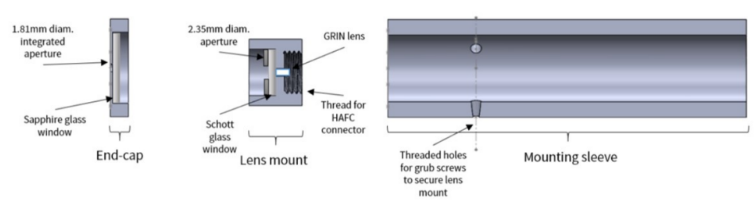
\includegraphics[width=0.8\textwidth]{Figures/collimator_schematic.png}
    \caption{Collimator schematic including the end-cap, lens mount and mounting sleeve structures.}
    \label{fig:collimator_schematic}
\end{figure}

 Because the collimated beams mean that there is no overlap of beam spots, there can be measurements of the water scattering and absorption coefficients made that are position dependent, allowing for an observation of how the water parameters depend on depth in the tank. A narrow beam spot means that more direct light is excluded from the analysis, allowing for better measurements of scattered light.

\subsubsection{The Diffuser Optic}

The diffuser optic is a wide angled beam with a opening half-angle of 40 degrees, allowing for more PMT coverage in the detector, therefore enabling measurements of PMT properties, and measurements of light attenuation length in water. Figure \ref{fig:diffuser_photo} shows a photograph of one of the diffusers used, and one of the diffuser ball enclosures. The enclosure is made of high grade stainless steel and using a chemical and water resistant epoxy resin, all the components were ensured to be watertight. 

\begin{figure}
    \centering
    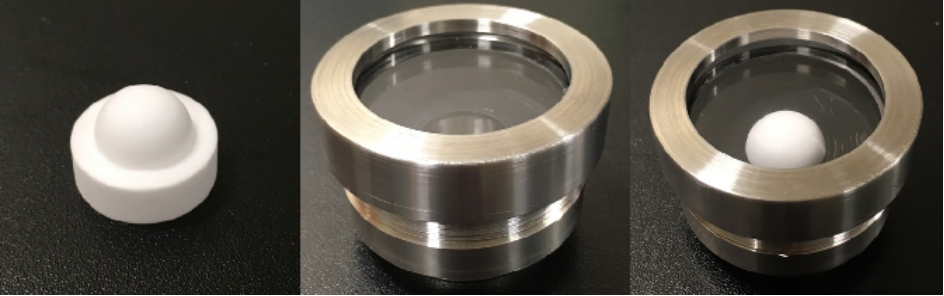
\includegraphics[width=0.7\textwidth]{Figures/diffuser_photo.png}
    \caption{Photograph of the diffuser by itself (left), empty diffuser enclosure (centre) and diffuser inside enclosure (right).}
    \label{fig:diffuser_photo}
\end{figure} 

\subsubsection{Bare Fibre and Optical Plate}

The bare fibre injector are 1 mm step index fibres, and are approximately 20 cm in length and are used for validation purposes with the bare fibres in the Korean optical calibration system. These short fibres are screwed into the back end of the optical plate that the collimator and diffuser optics are mounted on, shown in Figure \ref{fig:optical_plate}.

\begin{figure}
    \centering
    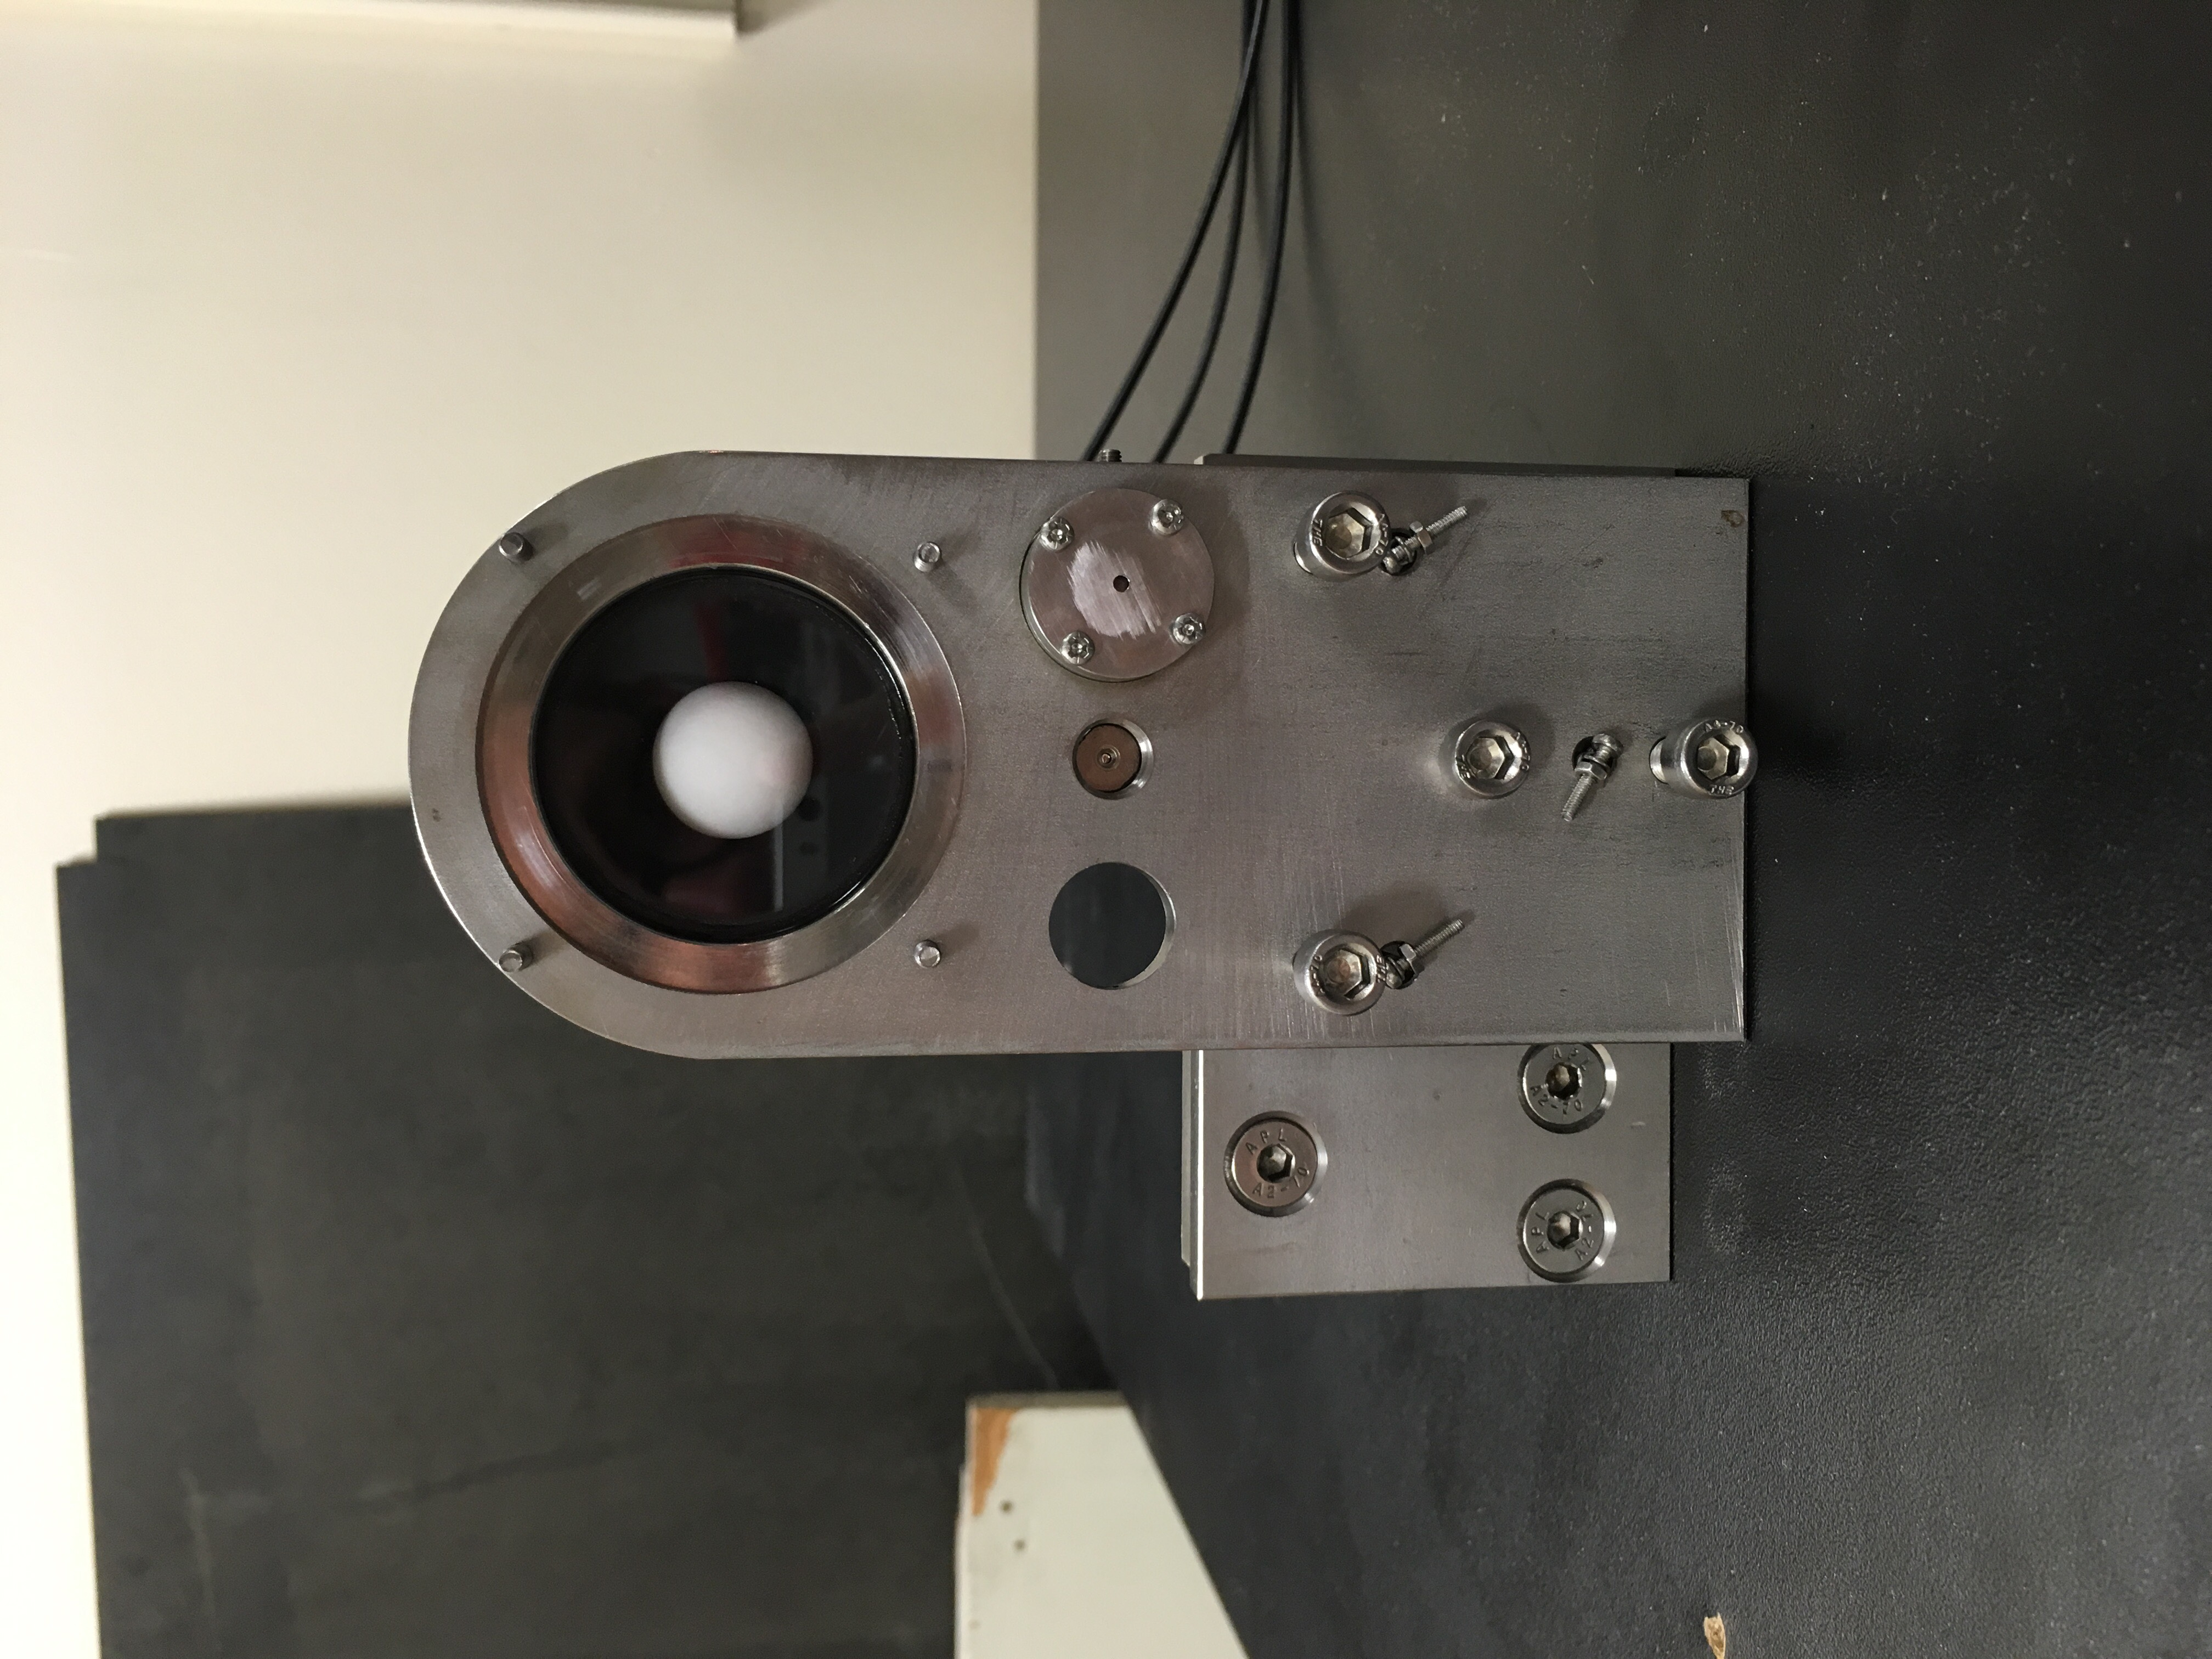
\includegraphics[width=0.7\textwidth, angle =270]{Figures/optical_plate.jpg}
    \caption{Photograph of the optical plate which houses the different optics.}
    \label{fig:optical_plate}
\end{figure}


\section{Optics test stand measurements}

In order to test the collimator and diffuser optics, measurements of the angular distributions were made using diffuser and collimator test-stands. These would measure angular distributions of the light intensity. For the diffuser test-stand the angular distribution of the light output was measured using the setup shown in Figure \ref{fig:diffuser_test_stand}. This test stand setup for the diffuser optics consists of a test diffuser ball placed inside a diffuser enclosure, a rotation stage which allows for the movement of the diffuser between -40 and 40 degrees, and a PMT used for pulse intensity measurement set up 250 mm away from the diffuser. An optical fibre couples the diffuser under test to a laser set to a wavelength of 450 nm. 


\begin{figure}
    \centering
    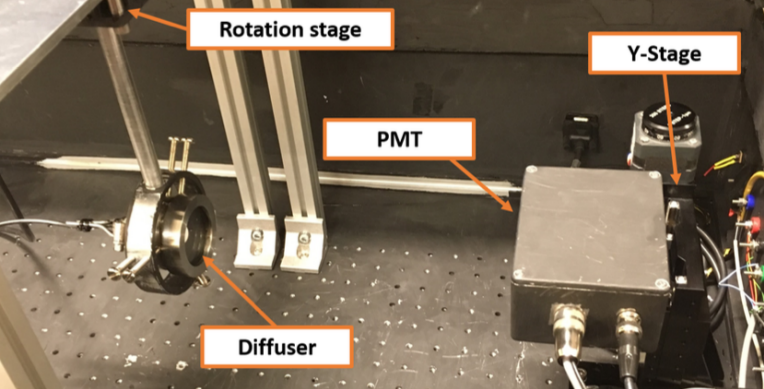
\includegraphics[width=0.7\textwidth]{Figures/diffuser_test_stand.png}
    \caption{Setup of the diffuser test stand provided by Warwick University}
    \label{fig:diffuser_test_stand}
\end{figure}

Figure \ref{fig:diffuser_TF1} shows distributions provided by this test stand data which are preliminary fits made by ROOT to the light profiles for the diffuser. 

\begin{figure}[!htbp]
    \centering
    
    \caption{Light profiles for the diffuser optics provided by The University of Warwick}\label{fig:diffuser_TF1}
    
    \subfloat[]{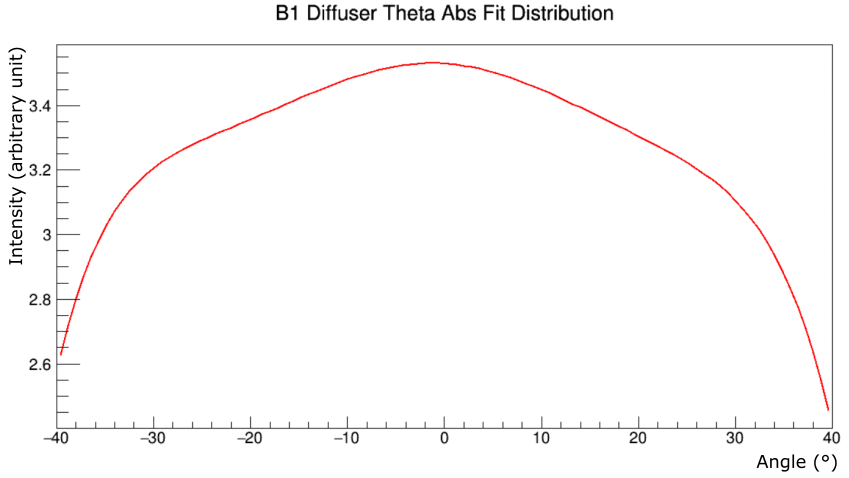
\includegraphics[width=0.49\textwidth]{Figures/B1_diffuser_fit.PNG}}\hfill
    \subfloat[]{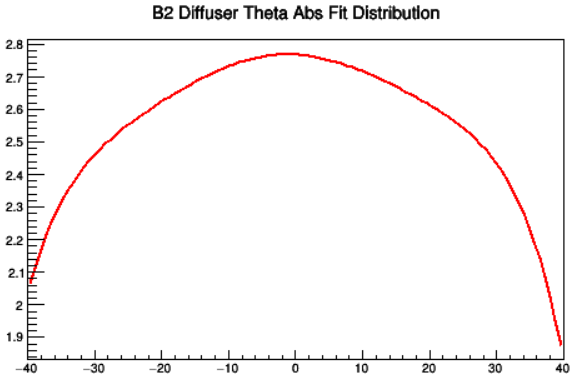
\includegraphics[width=0.49\textwidth]{Figures/B2_diffuser_fit.PNG}}\par
    \subfloat[]{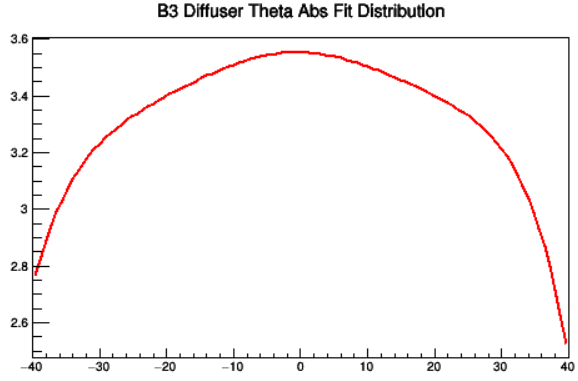
\includegraphics[width=0.49\textwidth]{Figures/B3_diffuser_fit.PNG}}\hfill
    \subfloat[]{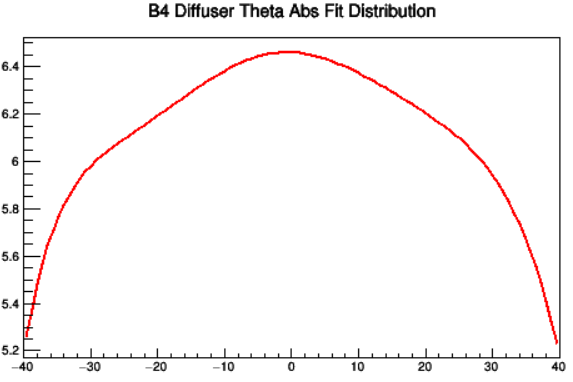
\includegraphics[width=0.49\textwidth]{Figures/B4_diffuser_fit.PNG}}\par
    \subfloat[]{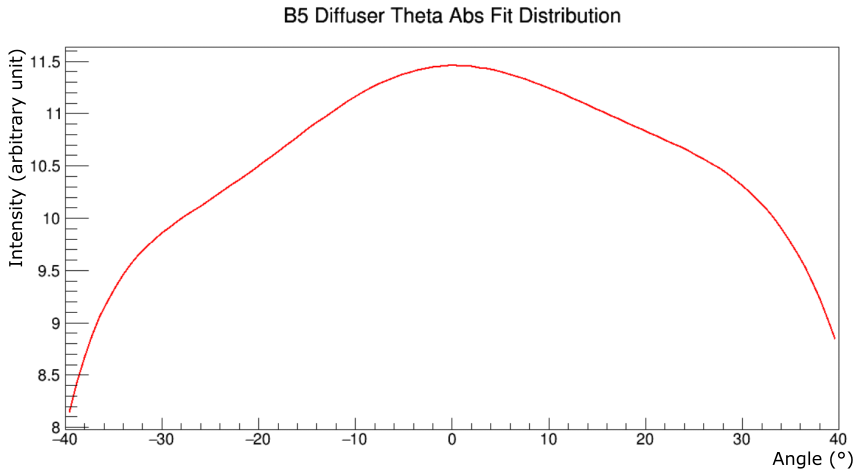
\includegraphics[width=0.49\textwidth]{Figures/B5_diffuser_fit.PNG}}
    
\end{figure}

The setup for the collimator test stand at the University of Warwick is shown in Figure \ref{fig:coll_test_stand} and captures the beam cross section by moving a CMOS camera along the beam width. 

\begin{figure}
    \centering
    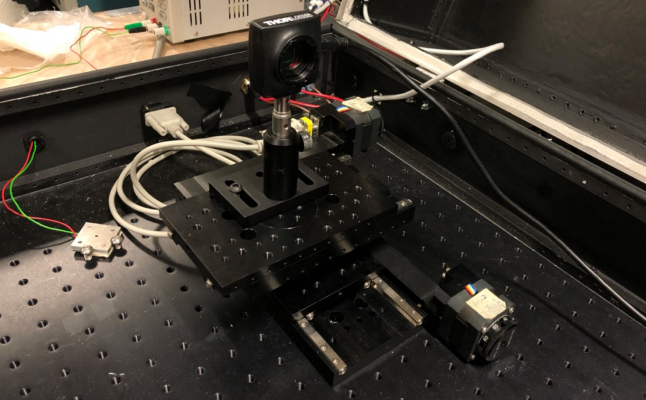
\includegraphics[width=0.7\textwidth]{Figures/coll_test_stand.png}
    \caption{Setup of the collimator test stand provided by Warwick University}
    \label{fig:coll_test_stand}
\end{figure}

Figure \ref{fig:collimator_TF1} shows fits made by ROOT to the light profiles for the collimator. The angular distributions shown give the distribution of the polar angle in degrees of light intensity which are relative to the virtual position from which the light cone originates, averaged over all the orientations of the azimuthal angle. 

\begin{figure}[!htbp]
    \centering
    
    \caption{Light profiles for the collimator optics provided by The University of Warwick}\label{fig:collimator_TF1}
    
    \subfloat[]{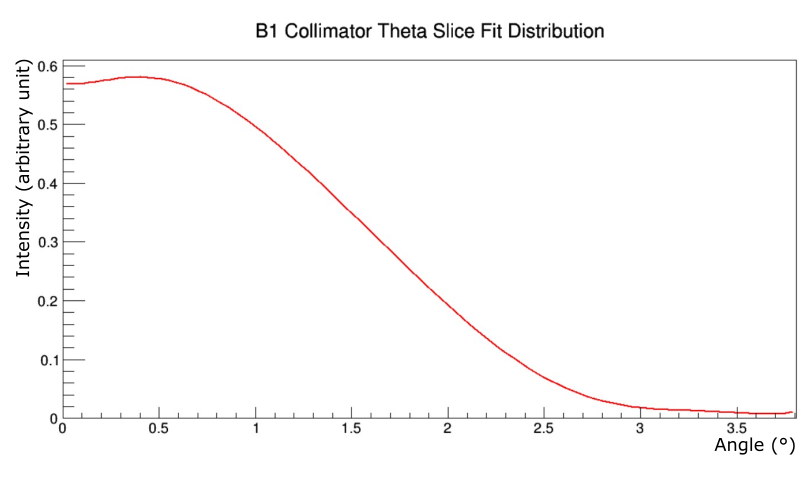
\includegraphics[width=0.49\textwidth]{Figures/B1_collimator_fit.PNG}}\hfill
    \subfloat[]{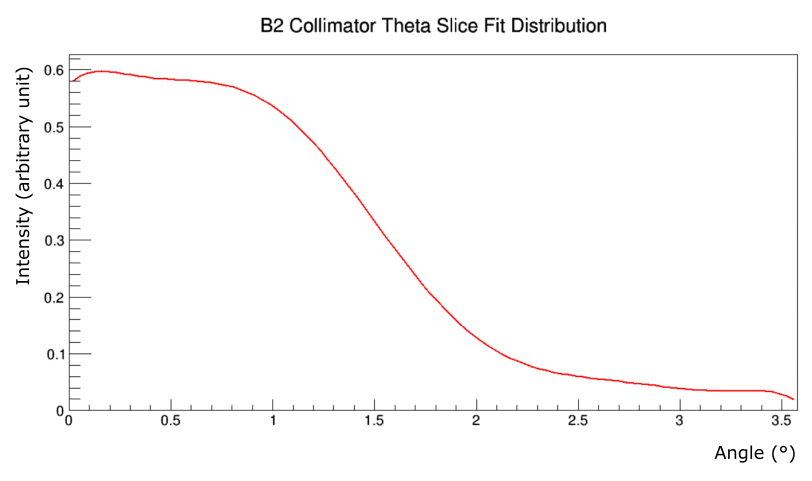
\includegraphics[width=0.49\textwidth]{Figures/B2_collimator_fit.PNG}}\par
    \subfloat[]{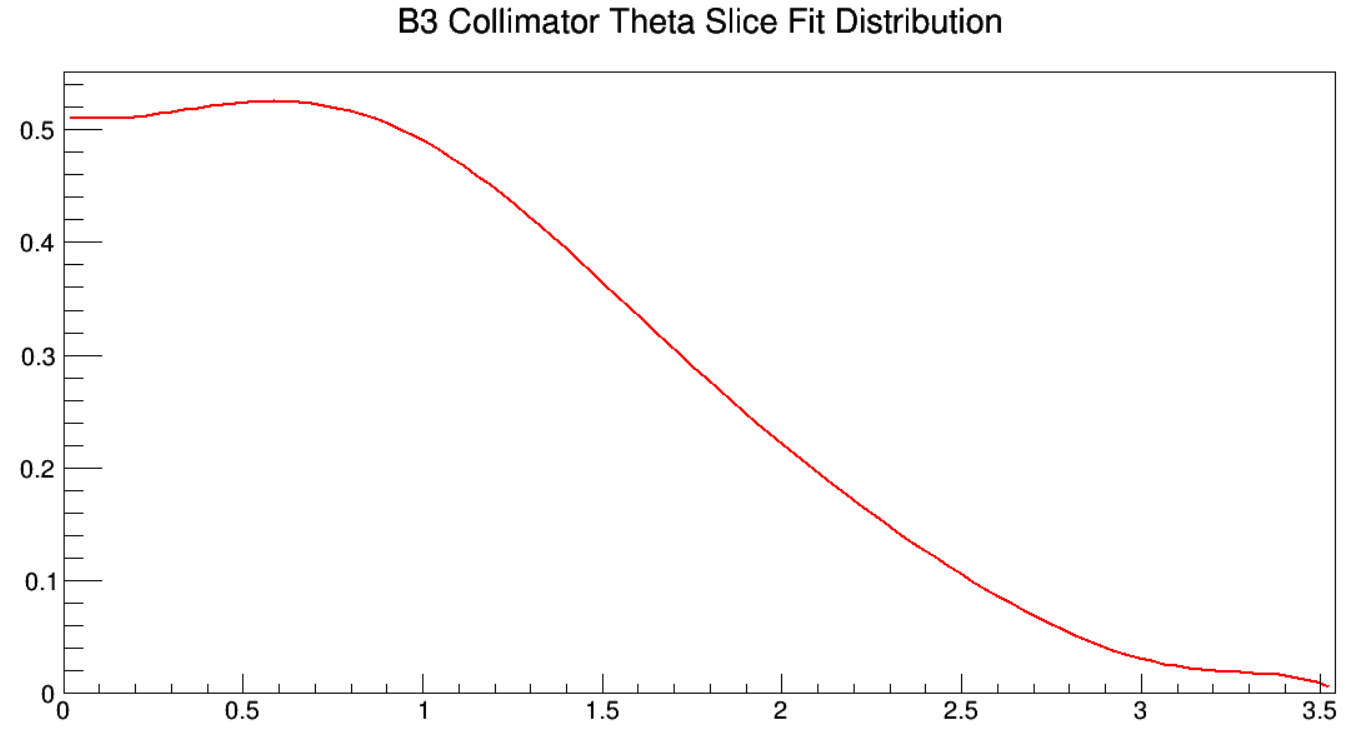
\includegraphics[width=0.49\textwidth]{Figures/B3_collimator_fit.PNG}}\hfill
    \subfloat[]{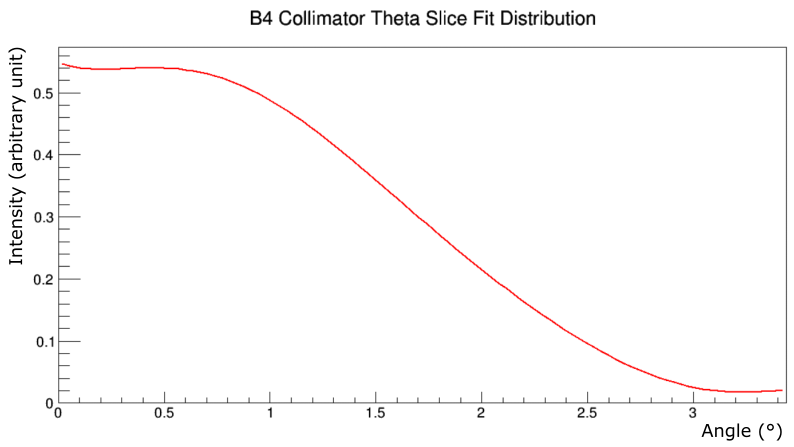
\includegraphics[width=0.49\textwidth]{Figures/B4_collimator_fit.PNG}}\par
    \subfloat[]{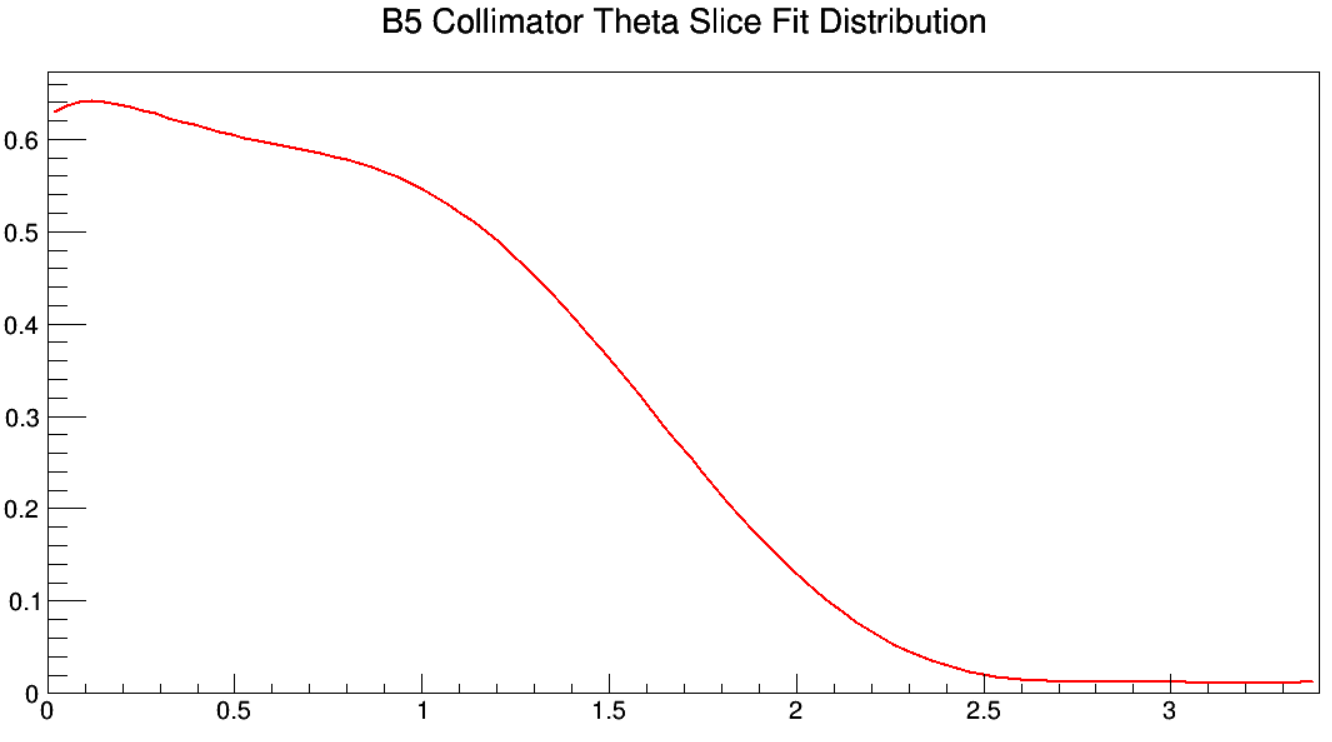
\includegraphics[width=0.49\textwidth]{Figures/B5_collimator_fit.PNG}}
\end{figure}





\section{First commissioning data from UKLI}

In September of 2019 and November of 2019 two sets of test data were taken of the collimator, the diffuser and the bare fibre optic (the B2 bare fibre) and using an event display developed by the University of Warwick, occupancy plots of the test data sets were produced. Figure \ref{fig:occupancy_coll} shows the occupancy plots for the collimator optic from the November 2019 dataset showing the beam spot inside the unrolled volume of the Super-Kamiokande detector. Similarly, Figure \ref{fig:occupancy_diffuser} shows the occupancy plots for the diffuser optic from the November 2019 dataset. The graph in the bottom right hand corner of the occupancy plots show the corrected time-of-flight plots for the PMT hits from the injector. Bare fibre data was taken, but used simply as a comparison to the output from the Korean system. 



\begin{figure}
    \centering
    
    \caption{Occupancy plot for the collimator optics from the UKLI November 2019 test run}
    \label{fig:occupancy_coll} 
    \subfloat[B1 collimator]{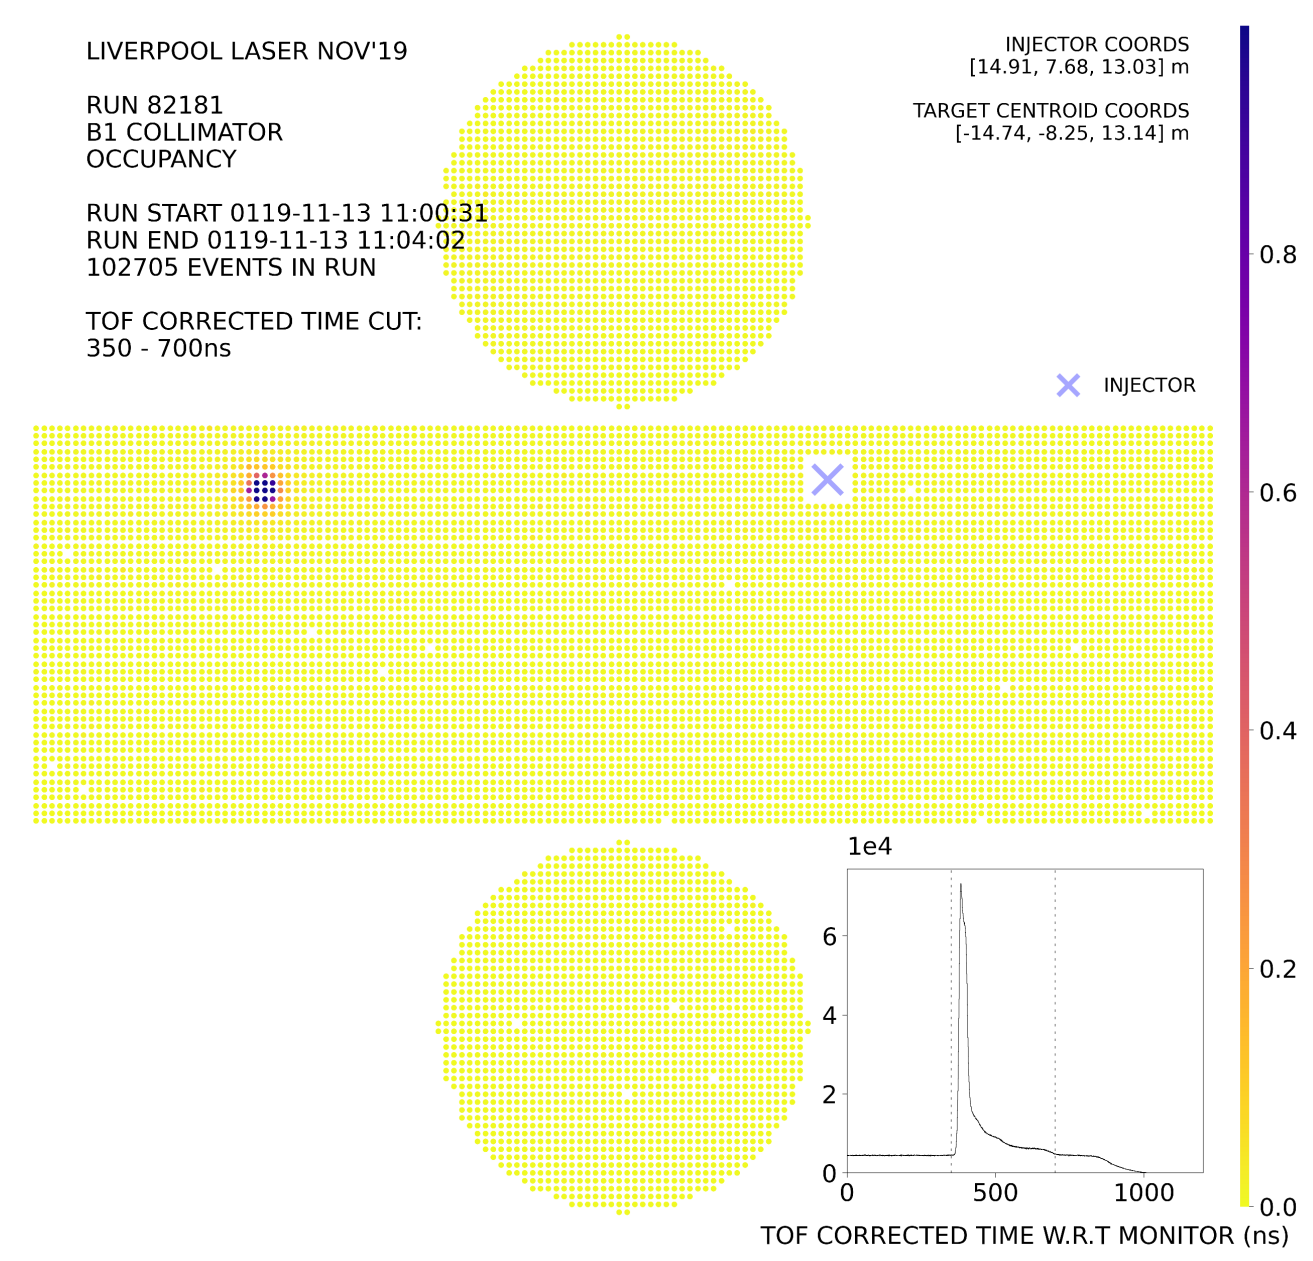
\includegraphics[width=0.49\textwidth]{Figures/B1_occupancy_coll.PNG}} \hfill
    \subfloat[B2 collimator]{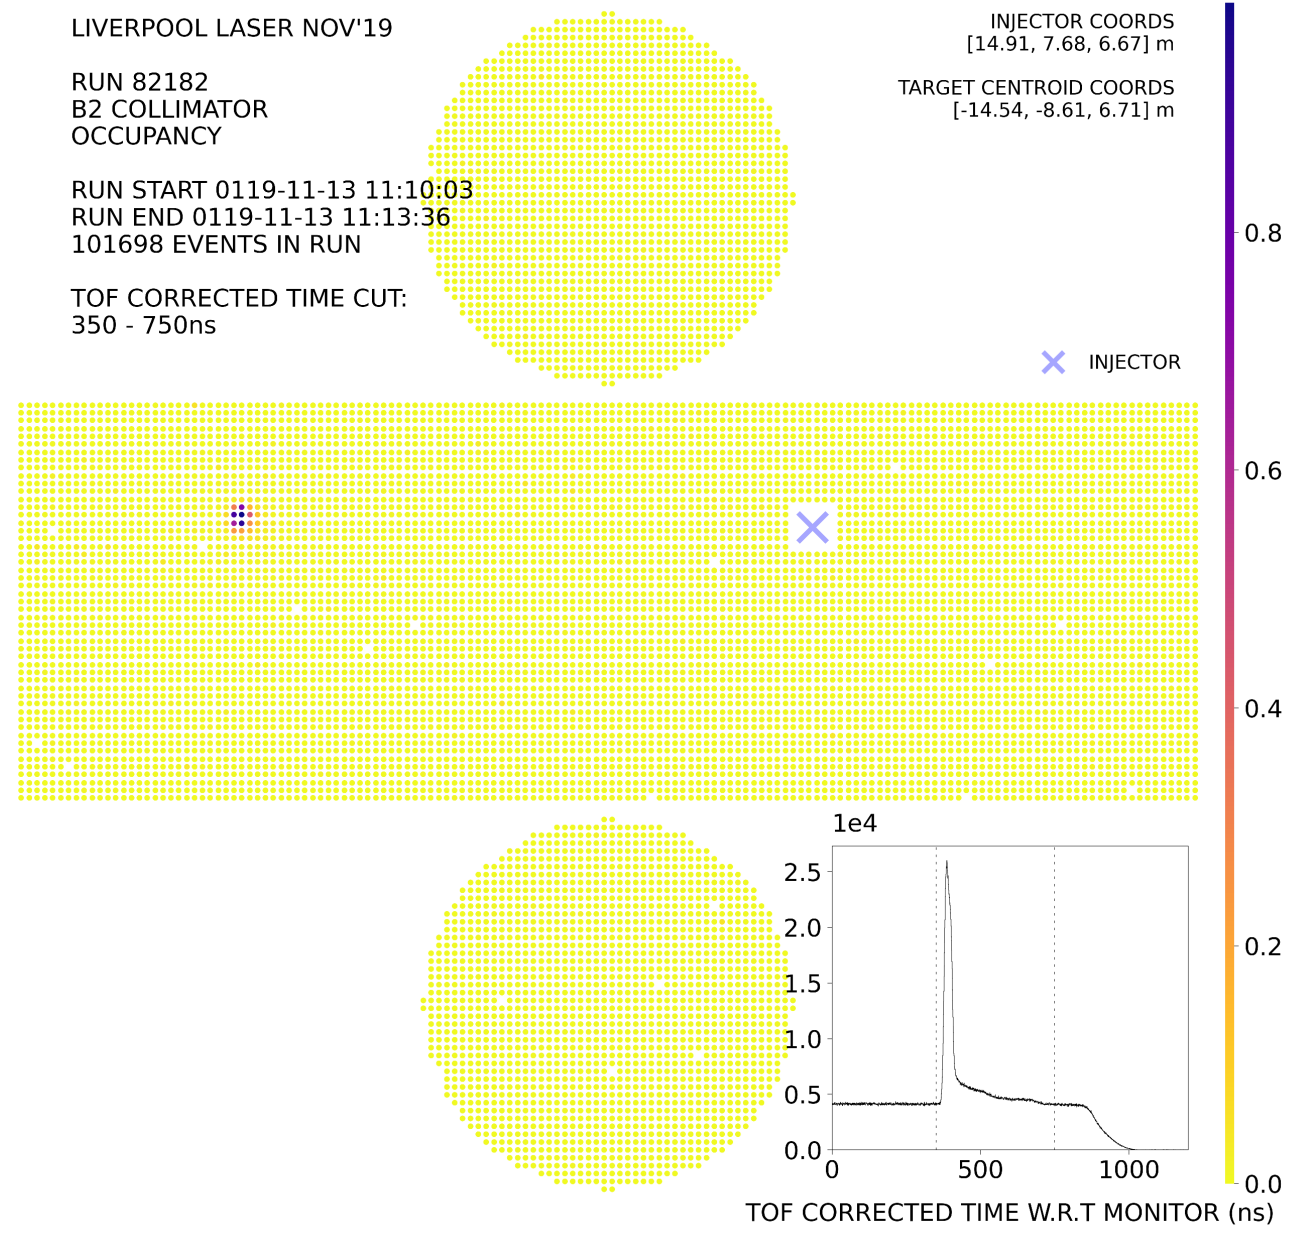
\includegraphics[width=0.49\textwidth]{Figures/B2_occupancy_coll.PNG}} \par
    \subfloat[B3 collimator]{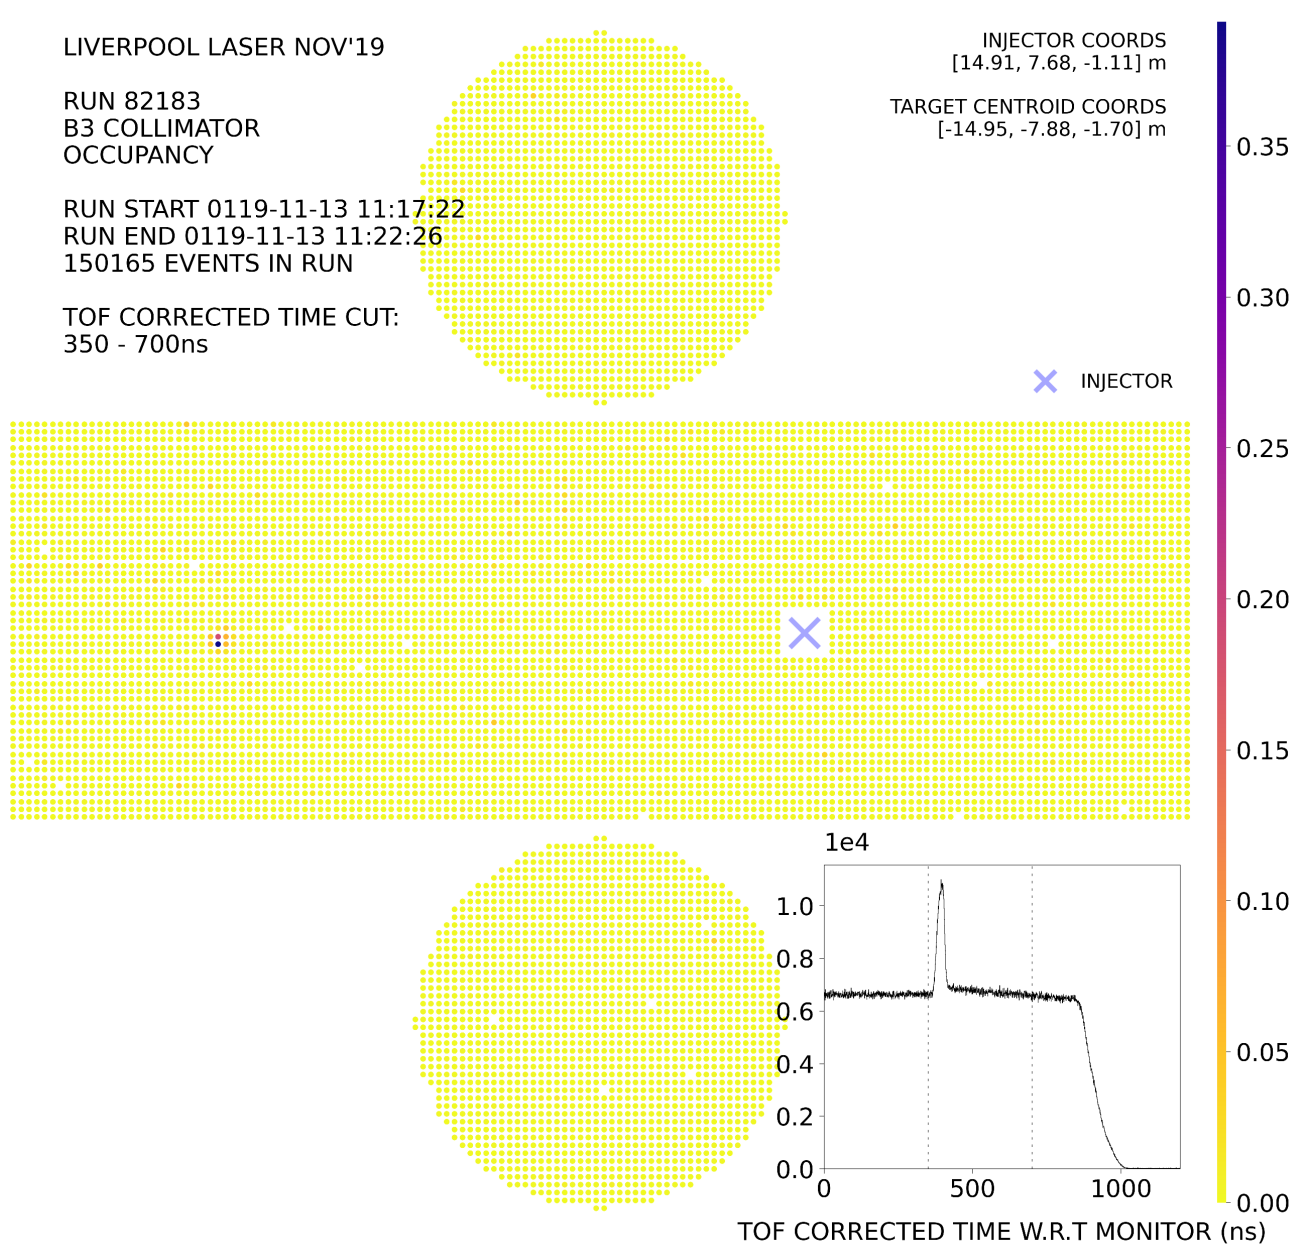
\includegraphics[width=0.49\textwidth]{Figures/B3_occupancy_coll.PNG}} \hfill
    \subfloat[B4 collimator]{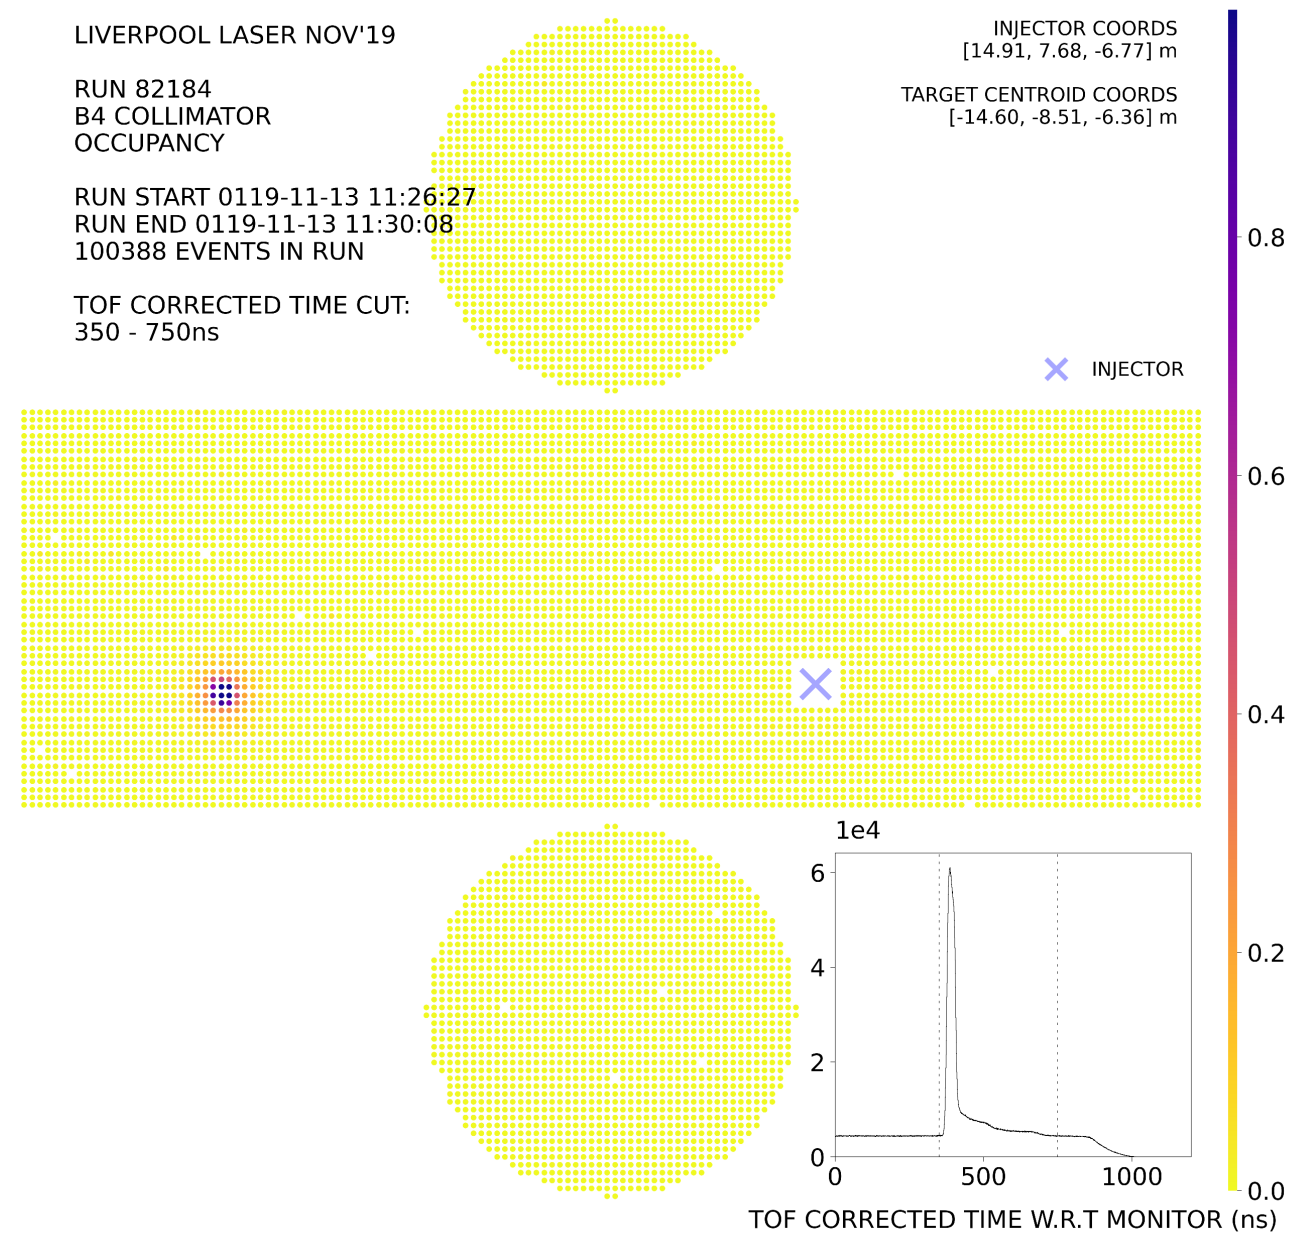
\includegraphics[width=0.49\textwidth]{Figures/B4_occupancy_coll.PNG}} \par
    \subfloat[B5 collimator]{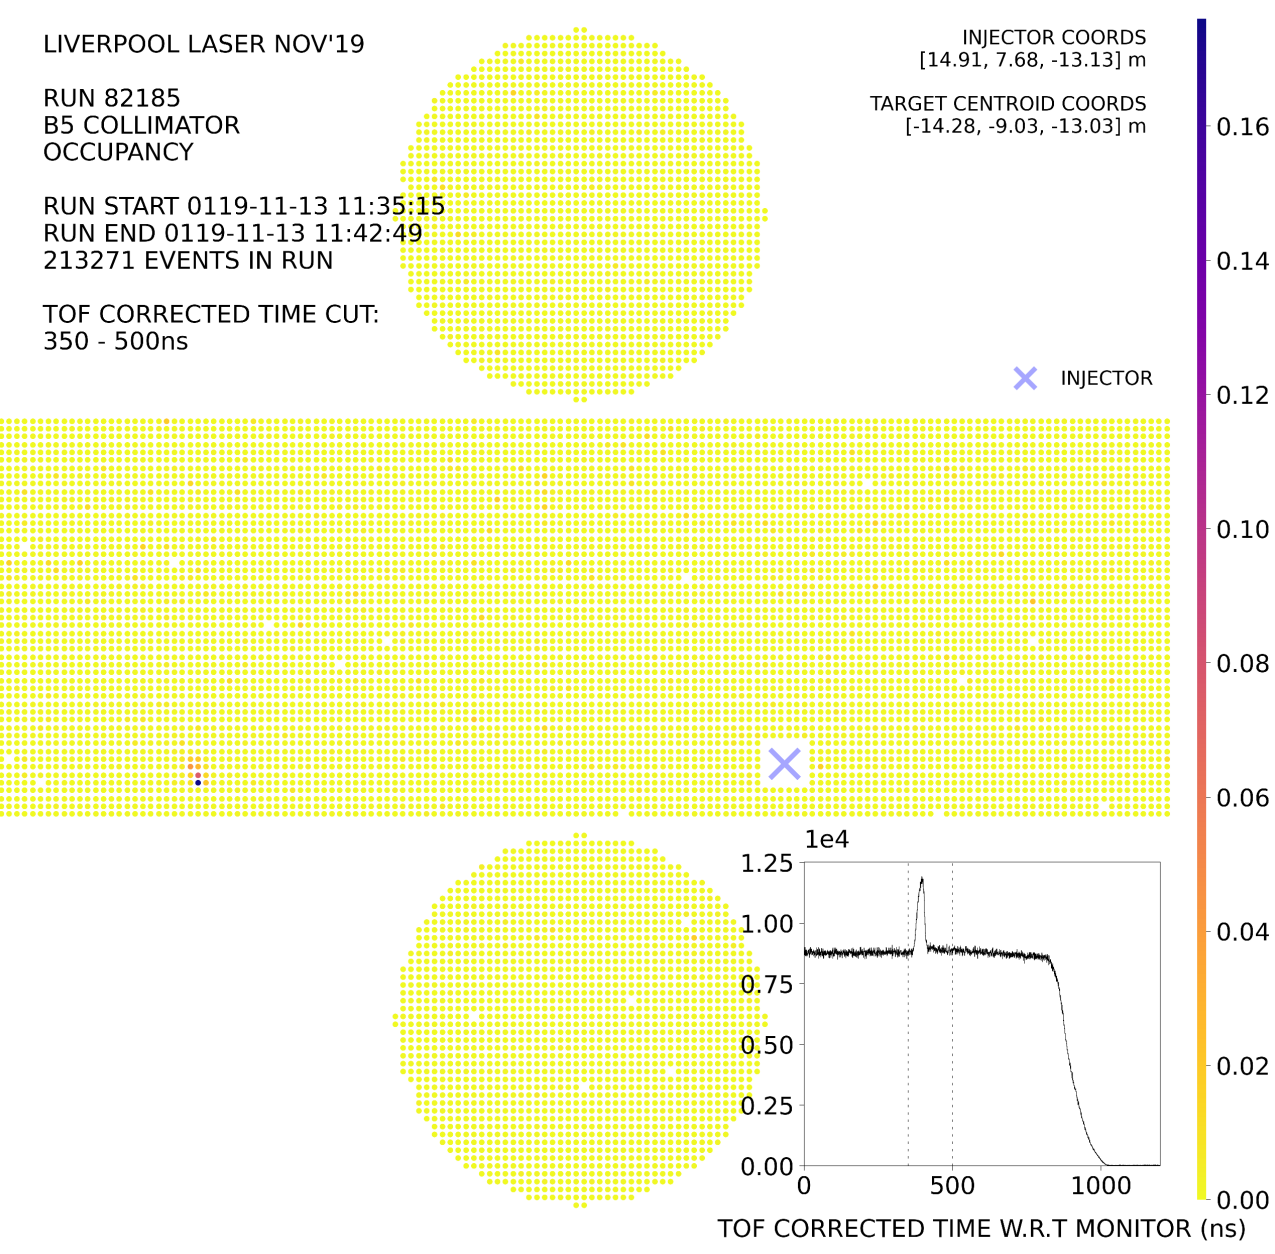
\includegraphics[width=0.49\textwidth]{Figures/B5_occupancy_coll.PNG}}
    \thisfloatpagestyle{empty}
\end{figure}


\begin{figure}
    \centering
    
    \caption{Occupancy plot for the diffuser optics from the UKLI November 2019 test run} \label{fig:occupancy_diffuser} 
    
    \subfloat[B1 diffuser]{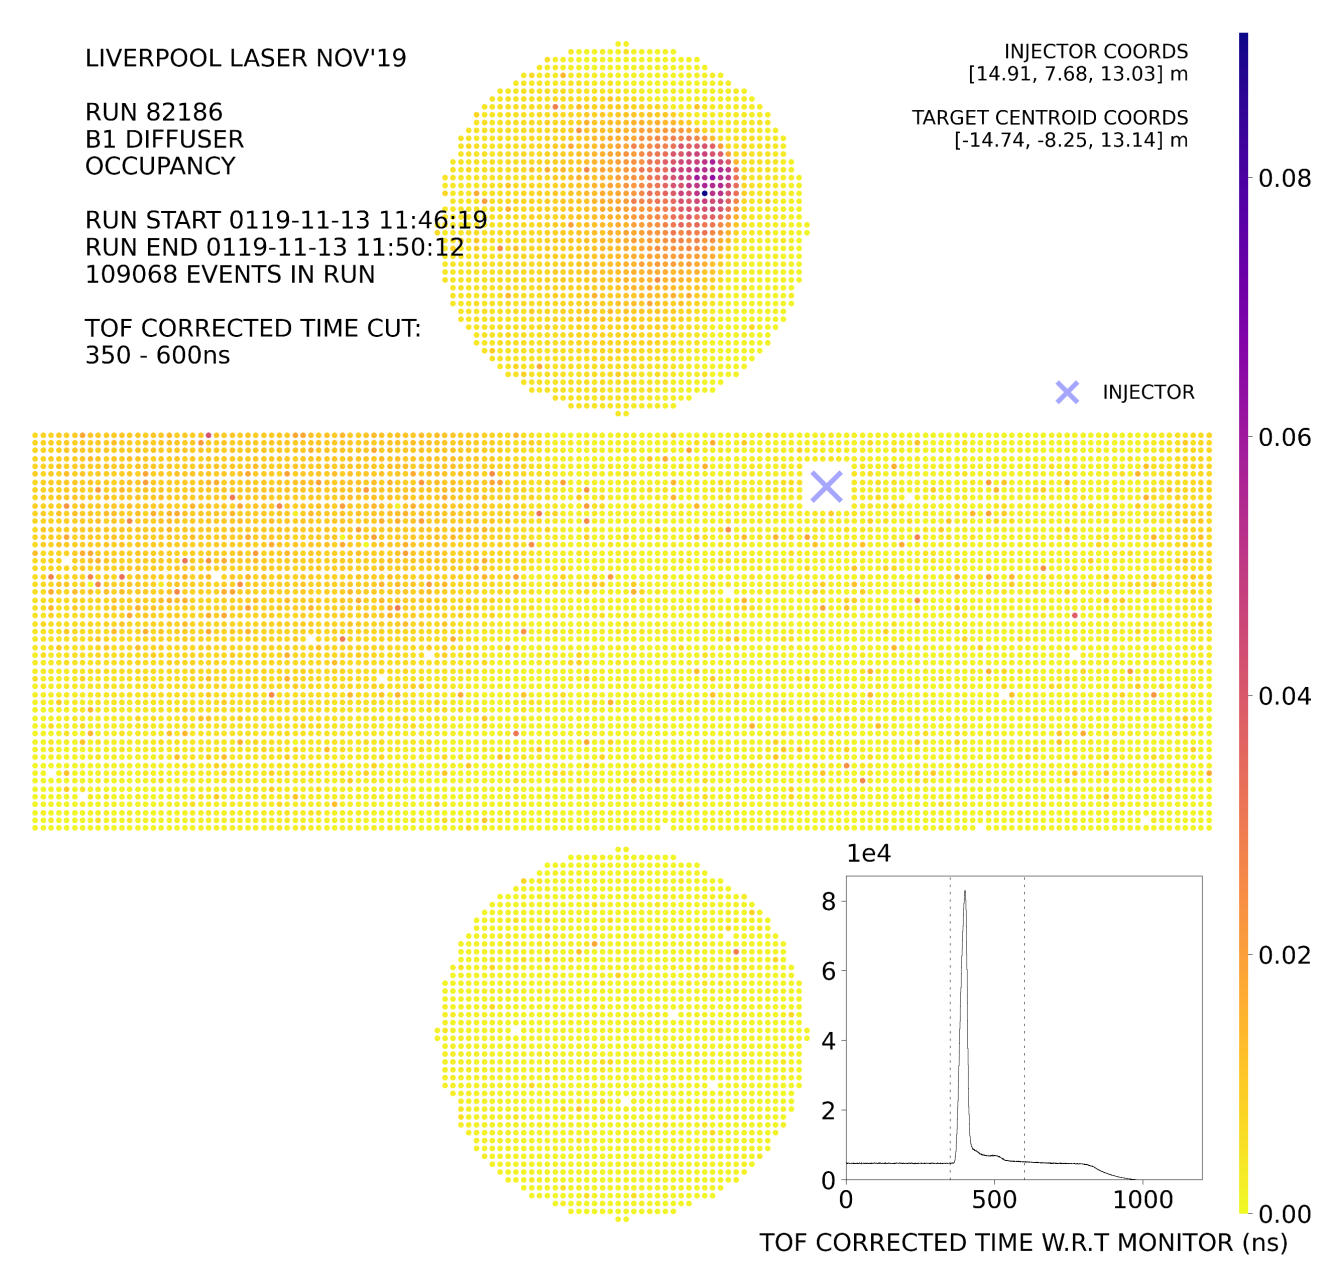
\includegraphics[width=0.49\textwidth]{Figures/B1_occupancy_diff.PNG}} \hfill
    \subfloat[B2 diffuser]{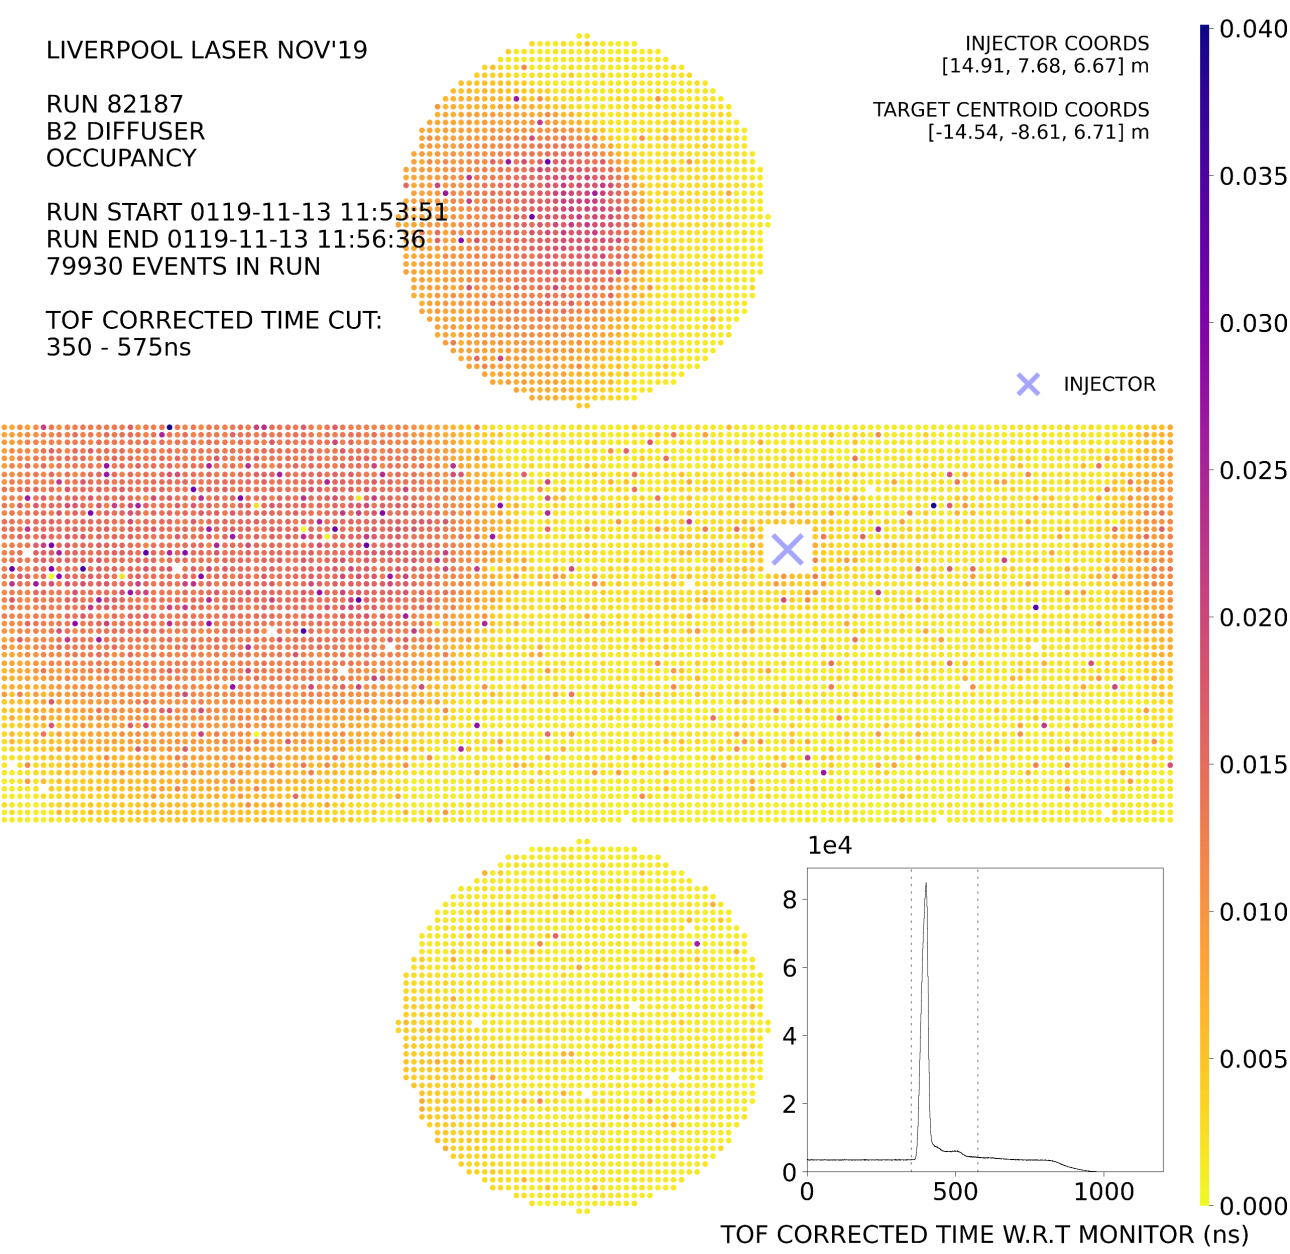
\includegraphics[width=0.49\textwidth]{Figures/B2_occupancy_diff.PNG}} \par
    \subfloat[B3 diffuser]{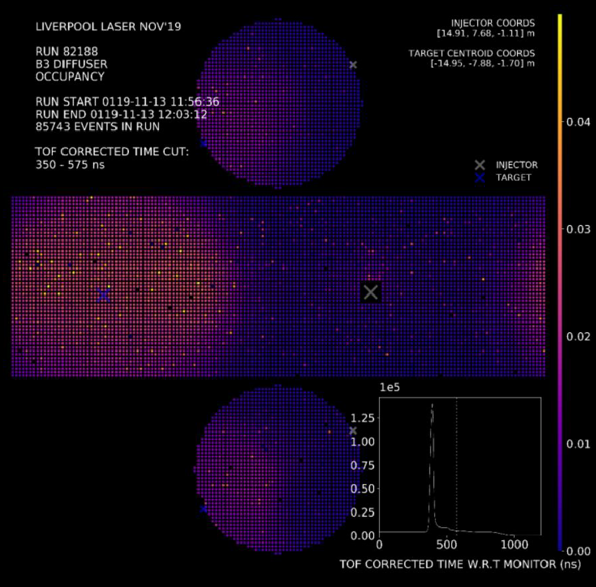
\includegraphics[width=0.49\textwidth]{Figures/B3_occupancy_diff.PNG}} \hfill
    \subfloat[B4 diffuser]{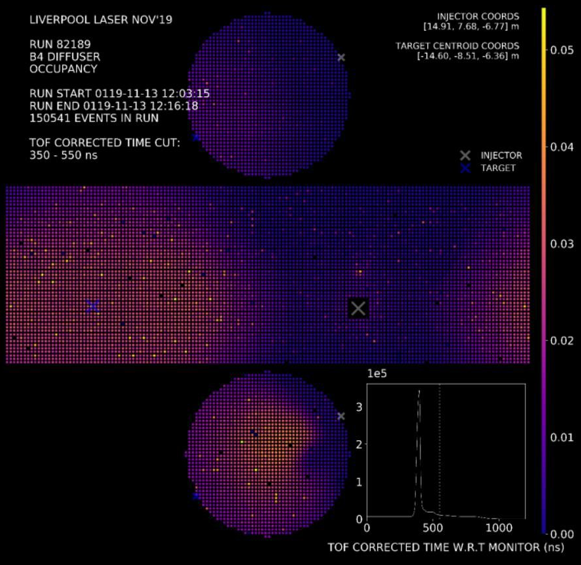
\includegraphics[width=0.49\textwidth]{Figures/B4_occupancy_diff.PNG}} \par
    \subfloat[B5 diffuser]{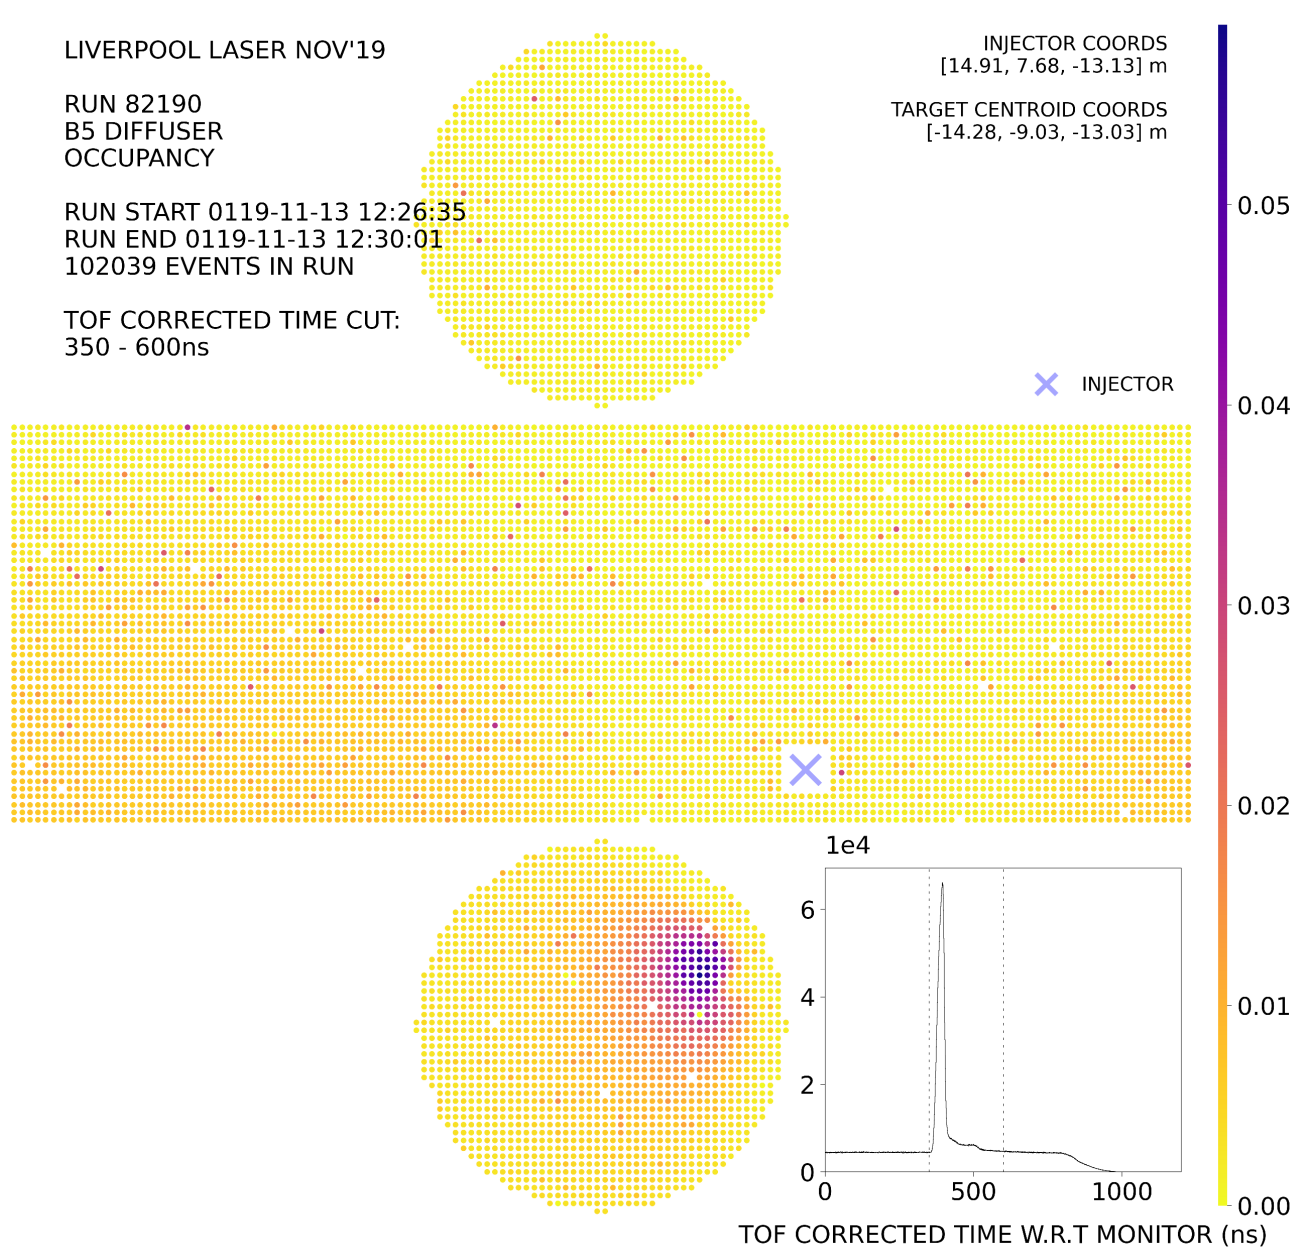
\includegraphics[width=0.49\textwidth]{Figures/B5_occupancy_diff.PNG}}
    
\end{figure}

The UKLI was also added to an ``autocalib'' system used for long term monitoring of the water parameters in Super-Kamiokande by the Korean laser system. In early 2020 the autocalib scheduler was modified to incorporate data taking by the UKLI system which was very useful for gadolinium loading calibration purposes but also in the longer term, it will be useful in the monitoring of daily/weekly water coefficient property measurements, investigation of depth dependence with respect to the water properties and PMT property calibration. Figure \ref{fig:autocalib} shows the schedule for autocalib, and the black dashed lines show the position of the UK barrel collimator and diffusers with respect to the other autocalib data taking streams. The horizontal blue line shows the length of the one autocalib cycle, which is about 4.6 seconds, with each UKLI optic taking about 3310 events per day.

\begin{figure}
    \centering
    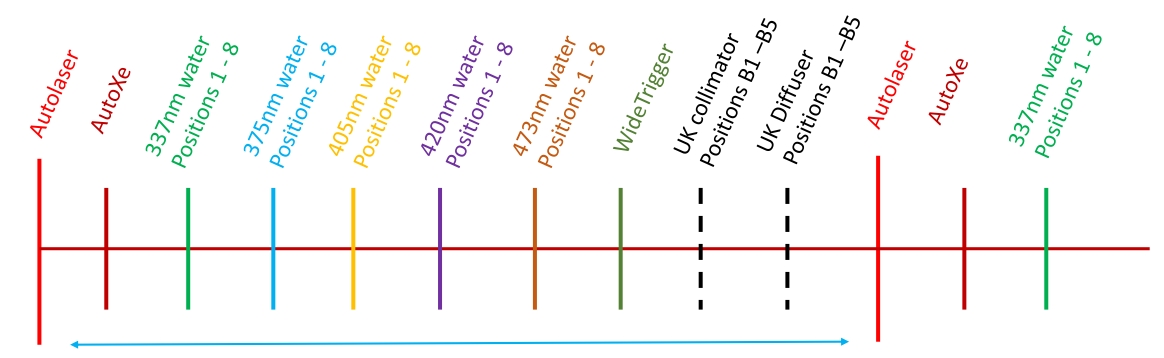
\includegraphics[width=0.8\textwidth]{Figures/autocalib.png}
    \caption{Schematic showing position of the UKLI in autocalib scheduler: the black dashed lines show the UKLI B1-B5 collimator and diffuser optics and the horizontal blue line shows the length of one autocalib cycle.}
    \label{fig:autocalib}
\end{figure}

Figures \ref{fig:B1_coll_diff_auto_July} shows the occupancy plots for autocalib data taken in July 2020, for the B1 collimator (left) and the B1 diffuser (right). From this point onwards all plots relating to the B2 - B5 injectors for both the collimators and diffusers will be shown in Appendix A. As can be seen in the text in the upper left hand corner, the number of events in the run is a lot less than the 100,000 events or so taken in the test runs, however they are more than sufficient for monitoring purposes.


\begin{figure}
    \centering
    
    \begin{minipage}{0.47\textwidth}
        \centering
        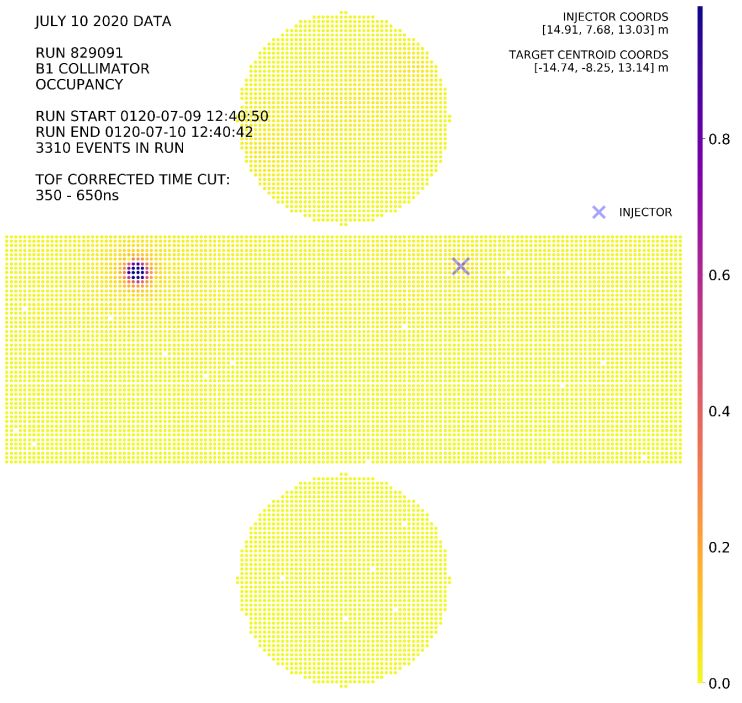
\includegraphics[width=\textwidth]{Figures/B1_occupancy_coll_auto.PNG} % first figure itself
        \caption{Occupancy plot for the B1 collimator optic from the UKLI Autocalib July 2020 run}
    \end{minipage}\hfill
    \begin{minipage}{0.47\textwidth}
        \centering
        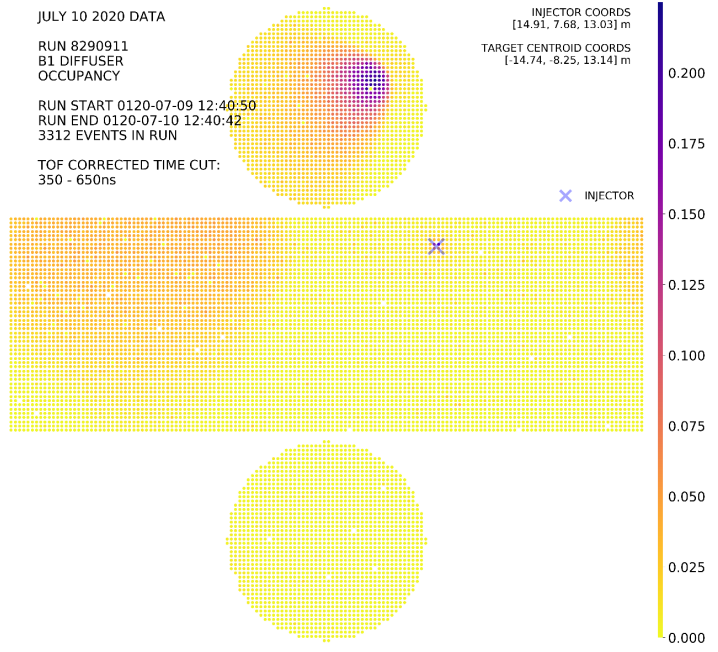
\includegraphics[width=\textwidth]{Figures/B1_occupancy_diff_auto.PNG} % second figure itself
        \caption{Occupancy plot for the B1 diffuser optic from the UKLI Autocalib July 2020 run}
        \label{fig:B1_coll_diff_auto_July}
    \end{minipage}
\end{figure}


\section{Implementation of UKLI in SK Simulation}
In order to simulate the data taken with the UKLI, SKDETSIM, the Super Kamiokande Detector Simulator was used. SKDETSIM uses GEANT3 (GEometry ANd Tracking 3) to simulate what the particles in each event would do inside the detector, and tracks the particle's trajectories and energy loss. Simulating the light injection from the UKLI system in SKDETSIM was done in a similar way to the Korean method of producing Monte Carlo: the same versions of the calibration scripts were used however, small modifications were made to them and to the version of SKDETSIM used to simulate the input photons from the system in the detector. The calibration software allows for the number of events and the number of injected photons to be set, in order to generate many Monte Carlo files with varying absorption, Rayleigh and Mie scattering parameters. 
\newline
Along with making sure the position of the injectors was set to that of the UKLI injectors (shown in Table \ref{table:UKLI_loc}), the opening angle of the injectors determined by the simulation had to be set to accomodate the fact that the injectors for the UKLI system now consisted of three different opening angles for the collimator, diffuser and bare fibre optics. Previously, to set the angle of the photons in the beam, a parameter relating to the width of the input injector beam was used (``SIGBM", standing for ``sigma of the beam"), and was produced using a Gaussian random number generator to produce the photon angle. However, an entirely new method of determining the opening angle of the beam was needed to include the information from the light profiles taken from the test stands at Warwick as the previous simulation included an algorithm for a 12$\degree$ opening angle that needed to be rewritten for our purposes for use with multiple optics. 

\begin{table}[htp]
    $$
\begin{array}{|c|c|c|c|c|c|}  
    \hline \hline{\text {UKLI Barrel Injector }} & {\text { x (cm)}} & {\text {y (cm)}} & {\text {z (cm)}}  \tabularnewline
    \hline \text { B1 } & 1490.73 & 768.14 & 1302.95 \\
    \hline \text { B2 } & 1490.73 & 768.14 & 666.2 \\
    \hline \text { B3 } & 1490.73 & 768.14 & -111.05 \\
    \hline \text { B4 } & 1490.73 & 768.14 & -676.65 \\
    \hline \text { B5 } & 1490.73 & 768.14 &  -1313.95 \\
    \hline \hline 
\end{array}
    $$
\caption{Theoretical barrel injector positions (x,y,z) of the UKLI injectors in cm} 
\label{table:UKLI_loc}
\end{table}

In order to validate the positions of the targets for the UKLI system, and the relationship between the width of the beam and the output angle, producing charge weighted histograms from UKLI test runs is very helpful. It allows us to explore the shape of the beam profile and intensity. Figures \ref{fig:charge_weighted_nov_sept_B1} and \ref{fig:charge_weighted_nov_sept_B4} shows the charge weighted z-profiles for the September and November 2019 datasets for the B1 and B4 collimator injectors, where the blue dashed line shows the expected target position. These are produced by selecting hit PMTs which are greater than 2 m away from the injector (to avoid including PMT hits from backscattered light), and filling the histogram with the z-position of the hit PMT and the number of hits the hit PMT recieves multiplied by the corrected charge from the PMT. The corrected PMT charge is calculated using Equation \ref{eq:gain_correction}, where the gain correction value is taken from official Super-Kamiokande gain tables. 

\begin{equation}
    q/(1 + gain)
\label{eq:gain_correction}
\end{equation}

\begin{figure}
    \centering
    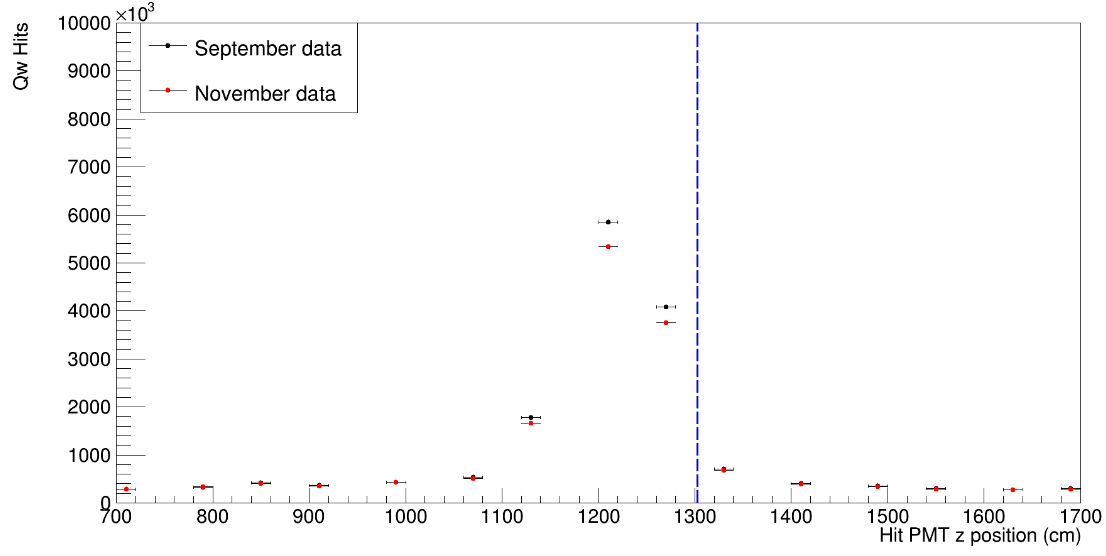
\includegraphics[width=0.9\textwidth]{Figures/charge_weighted_nov_sept_B1.PNG}
    \caption{Charge weighted z profile plots for the B1 collimator UKLI injector optic}
    \label{fig:charge_weighted_nov_sept_B1}
\end{figure}

\begin{figure}
    \centering
    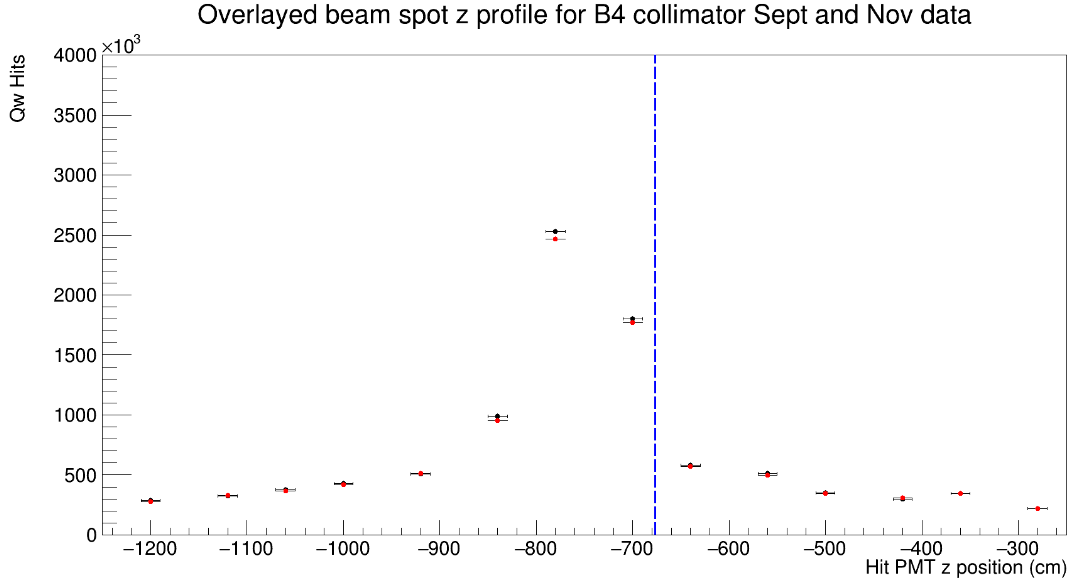
\includegraphics[width=0.9\textwidth]{Figures/charge_weighted_nov_sept_B4.PNG}
    \caption{Charge weighted z profile plots for the B4 collimator UKLI injector optic}
    \label{fig:charge_weighted_nov_sept_B4}
\end{figure}

The B1 and B4 collimator optics give the largest peaks in the charge weighted plots, while the B3 and B5 optics give the weakest peaks, practically indistinguishable from the background pedestal (even with the additional number of events taken during the November data taking runs.) These peaks of the distributions in these plots were used to calculate the actual injector positions, shown in Table \ref{table:actual_UKLI_injector_loc}. 

\begin{table}[htp]
    $$
\begin{array}{|c|c|c|c|c|c|}  
    \hline \hline{\text {UKLI Barrel Injector }} & {\text { x (cm)}} & {\text {y (cm)}} & {\text {z (cm)}}  \tabularnewline
    \hline \text { B1 } & 1490.73 & 768.14 & 1224 \\
    \hline \text { B2 } & 1490.73 & 768.14 & 742 \\
    \hline \text { B3 } & 1490.73 & 768.14 & -200 \\
    \hline \text { B4 } & 1490.73 & 768.14 & -747 \\
    \hline \text { B5 } & 1490.73 & 768.14 &  -1413 \\
    \hline \hline 
\end{array}
    $$
\caption{Actual barrel injector positions (x,y,z) of the UKLI injectors in cm} 
\label{table:actual_UKLI_injector_loc}
\end{table}

The charge weighted plots were used to validate the relationship between the opening angle of the injector beam in the Monte Carlo production calibration scripts by generating Monte Carlo scripts with varying values of the SIGBM parameter (while keeping the absorption and scattering parameters the same). Fitting the charge weighted profile plots with a Gaussian and using the position of the injector target and the edge of the beam spot, the opening angle of the beam in degrees could be determined. Figure \ref{fig:sigbm_angle_validation} shows the relationship between SIGBM and the opening angle of the beam in degrees. The width of the beam needed to be defined in order to do this however, and the standard beam radius definition is shown as in Figure \ref{fig:beam_width}. This schematic shows that the width of the beam was defined as using $1/e^2$ for the edge of the beam width, so it is taken as the point where the intensity drops to 0.135 of the Gaussian peak value.

\begin{figure}
    \centering
    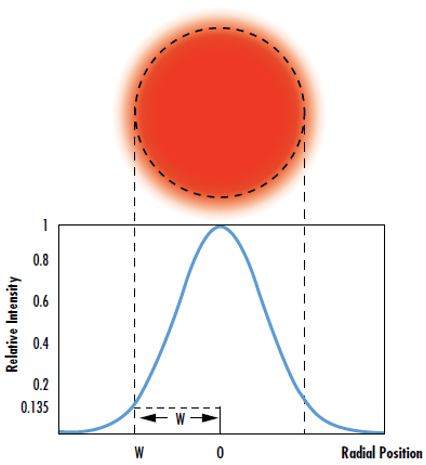
\includegraphics[width=0.7\textwidth]{Figures/beam_width.PNG}
    \caption{Schematic showing how the width of the MC beam was defined}
    \label{fig:beam_width}
\end{figure}

\begin{figure}
    \centering
    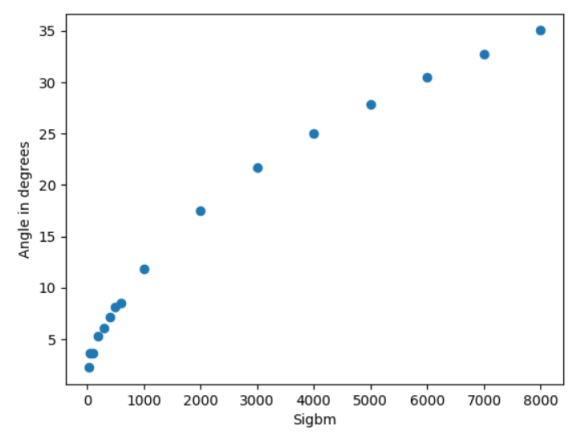
\includegraphics[width=0.7\textwidth]{Figures/sigbm_angle_validation.PNG}
    \caption{Plot of the sigbm parameter vs angle in degrees produced using calculation of the opening angle from the beam width}
    \label{fig:sigbm_angle_validation}
\end{figure}

After using the charge weighted hit plots to understand the SIGBM parameter and how the opening angle is generated by SKDETSIM more thoroughly, the next step involved using the profiles from the Warwick optic test stands (shown in Figures \ref{fig:collimator_TF1} and \ref{fig:diffuser_TF1}) in the production of this opening angle in the detector simulation. This was done by treating the profiles in Figures \ref{fig:collimator_TF1} and \ref{fig:diffuser_TF1} as Probablity Distribution Functions (PDFs) and using inverse transform sampling to make the detector simulation sample at random from it. Inverse transform sampling is a method for generating random numbers from any probability distribution by using the inverse of its cumulative distribution $F^{-1}(x)$. For continuous distributions, such as the results from the collimator and diffuser optics test stands, the algorithm for inverse transform sampling is simple. Firstly, a random variable $U$ is uniformly distributed between [0,1], and secondly the relation $X = F^{-1}_{x}(U)$ would then produce a distribution $X$ following the original probability distribution function, i.e. that of the original PDFs from the optics test stands. 

The first step is to produce the CDFs from the PDFs from the optic test stand profile tests. Figure \ref{fig:collimator_TF1} shows that the original fits to the collimator data did not reach 4 degrees, and as a result the PDFs produced needed to be linearly extrapolated from 3.5 degrees where the measurements cut off to reach 4 degrees. Figure \ref{fig:B1_PDF_CDF_coll} shows the PDFs and CDFs produced from the collimator data, and Figure \ref{fig:B1_PDF_CDF_diff} shows the PDFs and CDFs produced from the diffuser data. The CDFs are normalised with a max of one using min-max scaling.


\begin{figure}
    \centering
    
    \begin{minipage}{0.5\textwidth}
        \centering
        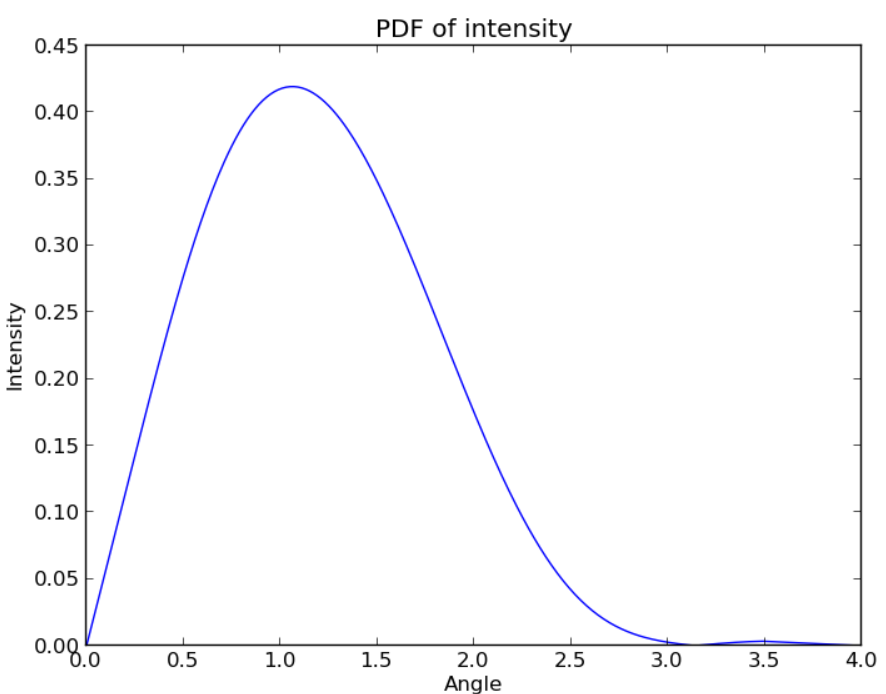
\includegraphics[width=\textwidth]{Figures/B1_coll_pdf.png} % first figure itself
        \caption{PDF for the B1 collimator}
    \end{minipage}\hfill
    \begin{minipage}{0.5\textwidth}
        \centering
        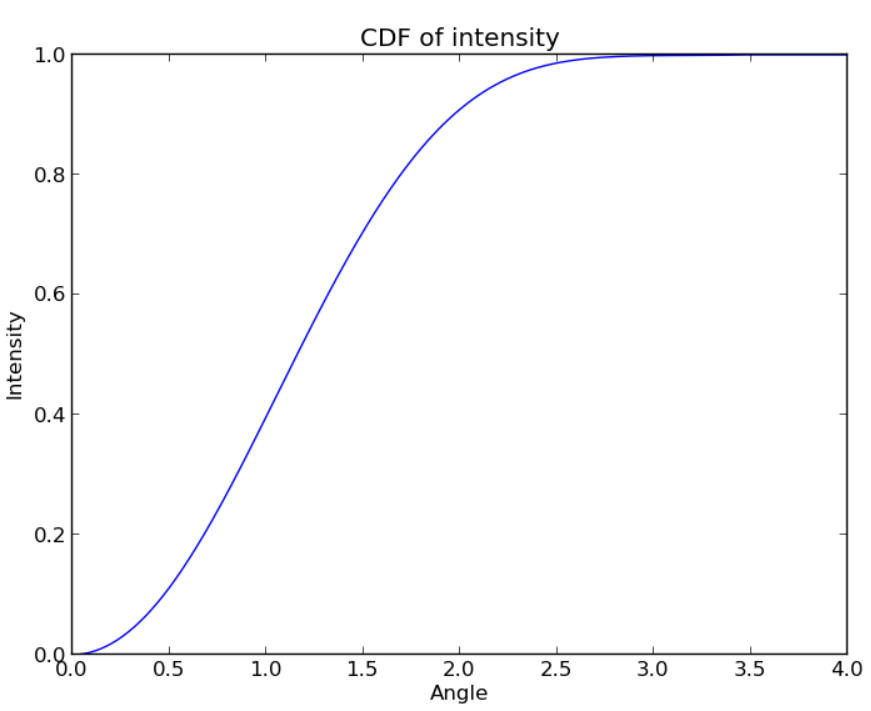
\includegraphics[width=\textwidth]{Figures/B1_coll_cdf.png} % second figure itself
        \caption{CDF for the B1 collimator }
        \label{fig:B1_PDF_CDF_coll}
    \end{minipage}
\end{figure}

\begin{figure}
    \centering
    
    \begin{minipage}{0.5\textwidth}
        \centering
        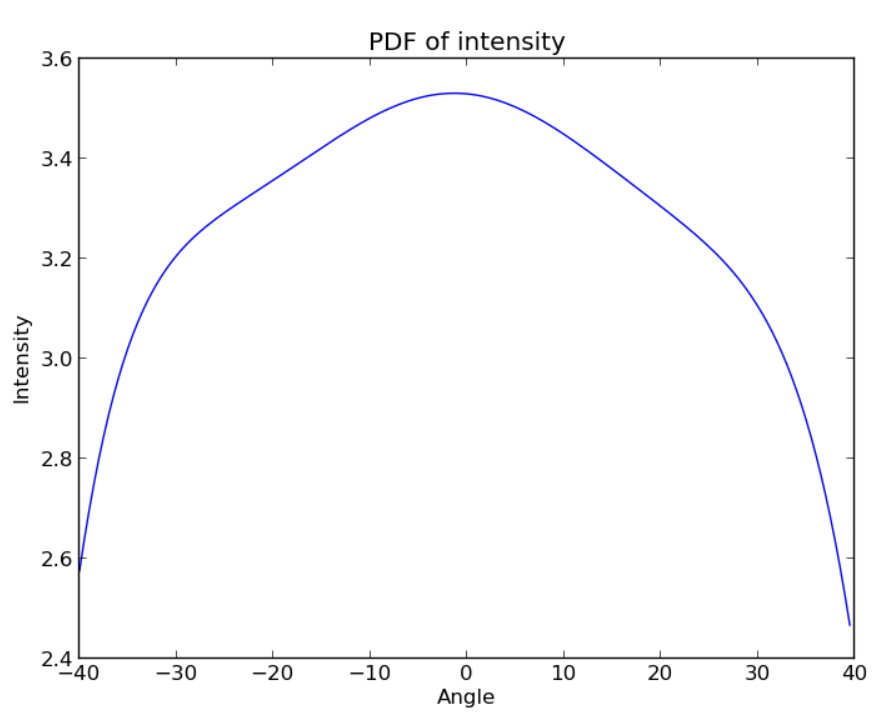
\includegraphics[width=\textwidth]{Figures/B1_diff_pdf.png} % first figure itself
        \caption{PDF for the B1 diffuser}
    \end{minipage}\hfill
    \begin{minipage}{0.5\textwidth}
        \centering
        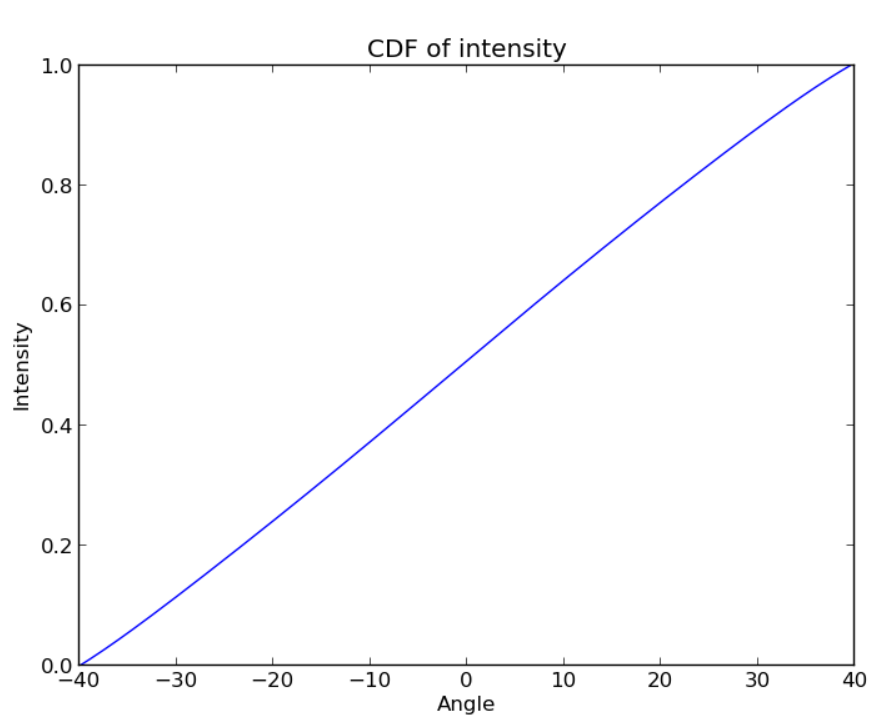
\includegraphics[width=\textwidth]{Figures/B1_diff_cdf.PNG} % second figure itself
        \caption{CDF for the B1 diffuser}
        \label{fig:B1_PDF_CDF_diff}
    \end{minipage}
\end{figure}


After producing the normalised CDFs, the inverse of these CDFs are calculated - Figure \ref{fig:B1_PDF_CDF_inv_coll} shows the comparison of the normalised CDF data for the B1 collimator (top sublot, shown in blue) and the polynomial fit to the CDF for the B1 collimator (top subplot, shown in red), and the inverse CDF function (bottom subplot shown in green) and the polynomial fit to this inverse CDF function (bottom subplot shown in purple). Figure \ref{fig:B1_PDF_CDF_inv_diff} shows the same plot for the B1 diffuser. 

\begin{figure}
    \centering
    \begin{minipage}{0.5\textwidth}
        \centering
        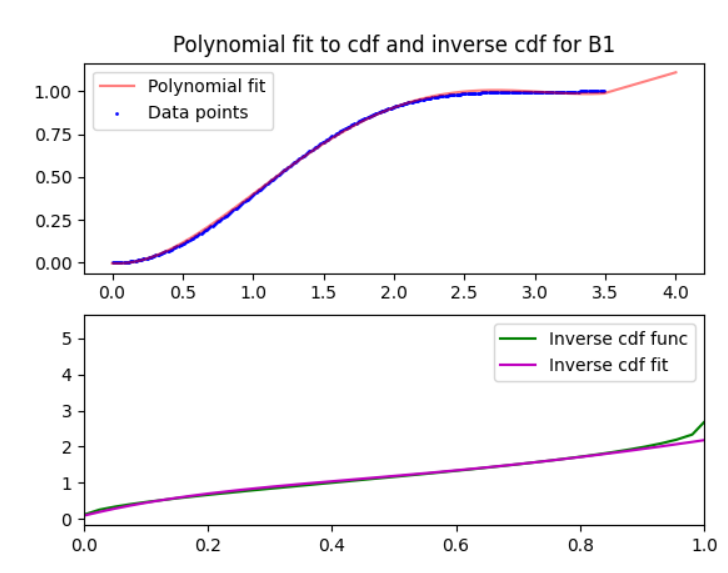
\includegraphics[width=\textwidth]{Figures/B1_inv_coll_cdf.png} % first figure itself
        \caption{Inverse CDF for the B1 collimator}
        \label{fig:B1_PDF_CDF_inv_coll}
    \end{minipage}\hfill
    \begin{minipage}{0.5\textwidth}
        \centering
        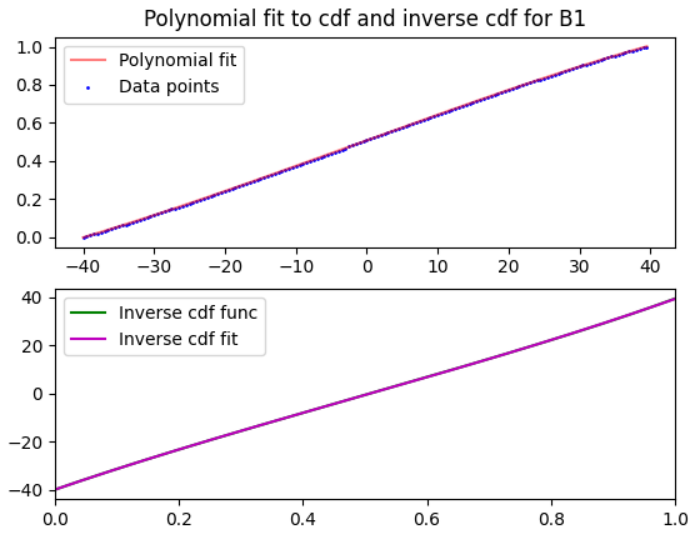
\includegraphics[width=\textwidth]{Figures/B1_inv_diff_cdf.png} % second figure itself
        \caption{Inverse CDF for the B1 diffuser}
        \label{fig:B1_PDF_CDF_inv_diff}
    \end{minipage}
\end{figure}


After producing the fits to the inverse cumulative distribution functions, these funtions were inputted into the detector simulation, SKDETSIM. Removing the SIGBM parameter from the calibration scripts meant there needed to be a new way with which to generate the angle at which the photons were produced in the simulation, and this is where the inverse transform sampling occurs for the relevant fit for the selected injector and optic type. Using the same event display used to produce the occupancy plots for the autocalib data and the test run data, occupancy plots of the Monte Carlo were produced. These are shown for the B1 - B5 collimators in Figure \ref{fig:ukli_mc_coll}, and for the B1 - B5 diffusers in Figure \ref{fig:ukli_mc_diff}. These MC were produced with the abs, ray and mie parameters in the calibration scripts set to 1.0, 1.0, and 1.0 (i.e. the current detector simulation values) and the top-bottom asymmetry parameter set to 7.598, which is the most recently tuned value of this parameter. Because the original profiles from the test stands were taken in air, adjustments were made so that the refractive index of the water in the detector was taken into account when implementing the inverse CDFs into the detector simulation. 

\begin{figure}[htp]
    \centering
    \caption{Monte Carlo simulations of the B1 - B5 collimator injectors}
    \label{fig:ukli_mc_coll}
    \begin{subfigure}{0.49\columnwidth}
    \centering
    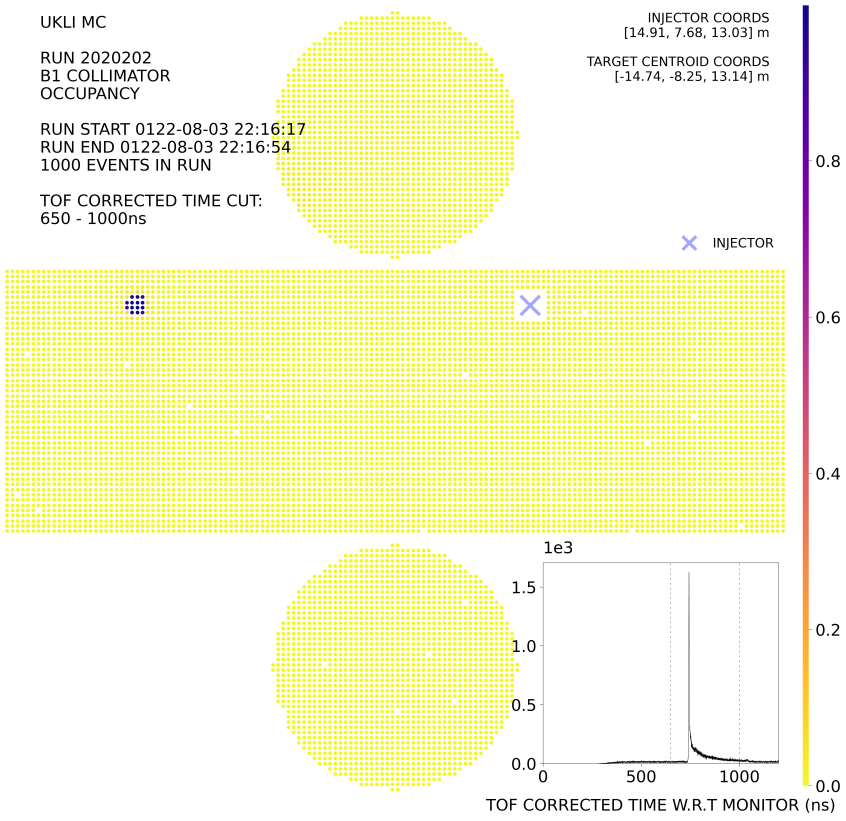
\includegraphics[width=0.9\textwidth]{Figures/ukli_mc_B1.PNG}
    \caption{B1 collimator UKLI MC}
    \label{fig:time1}
    \end{subfigure}\hfill
    \begin{subfigure}{0.49\columnwidth}
    \centering
    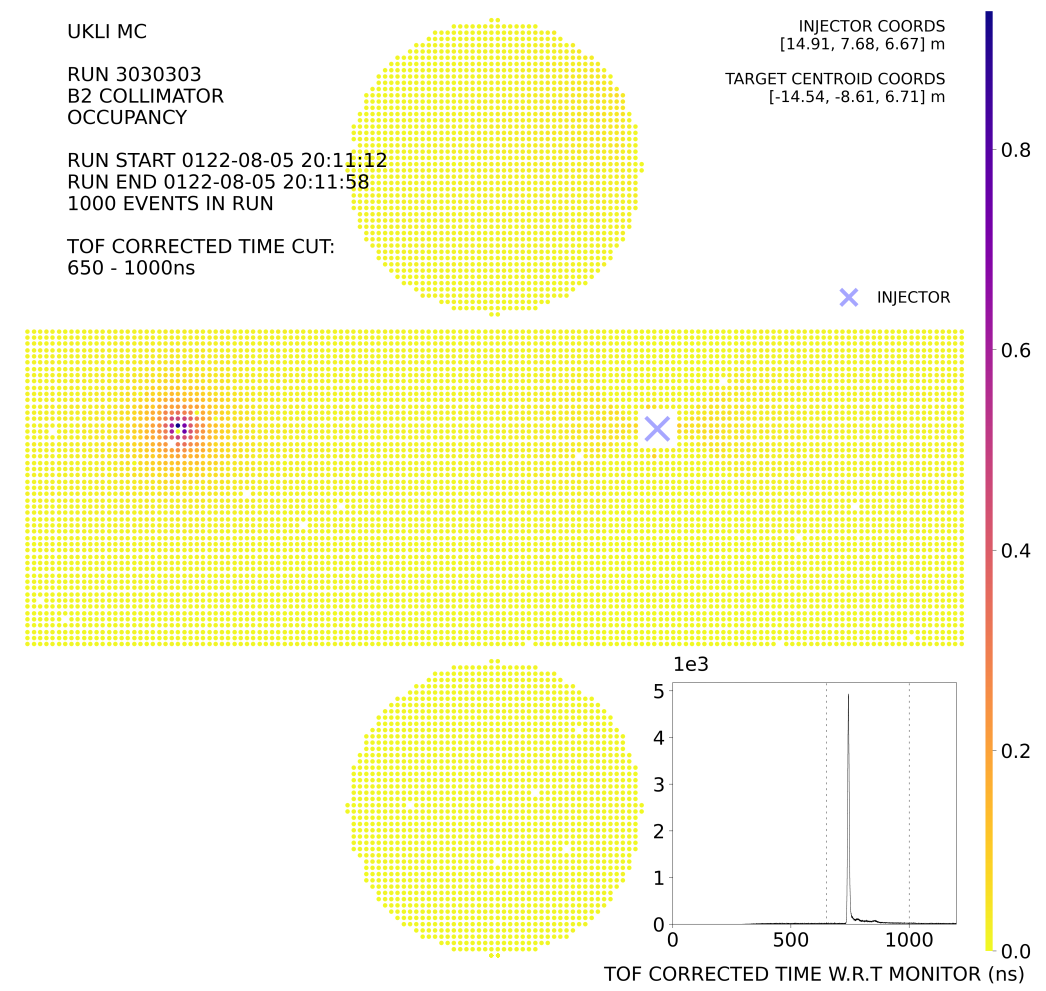
\includegraphics[width=0.9\textwidth]{Figures/ukli_mc_B2.PNG}
    \caption{B2 collimator UKLI MC}
    \label{fig:time2}
    \end{subfigure}
    
  
    \begin{subfigure}{0.49\columnwidth}
    \centering
    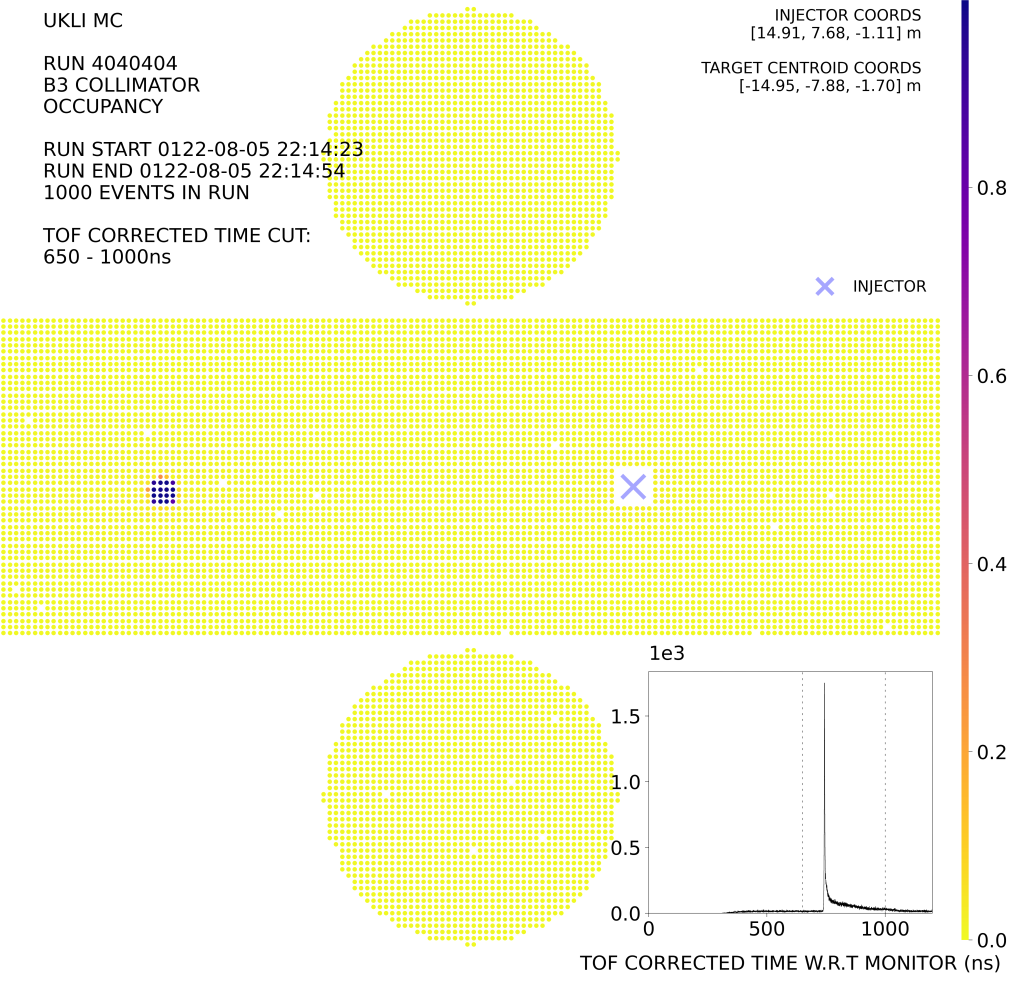
\includegraphics[width=0.9\textwidth]{Figures/ukli_mc_B3.PNG}
    \caption{B3 collimator UKLI MC}
    \label{fig:time3}
    \end{subfigure}\hfill
    \begin{subfigure}{0.49\columnwidth}
    \centering
    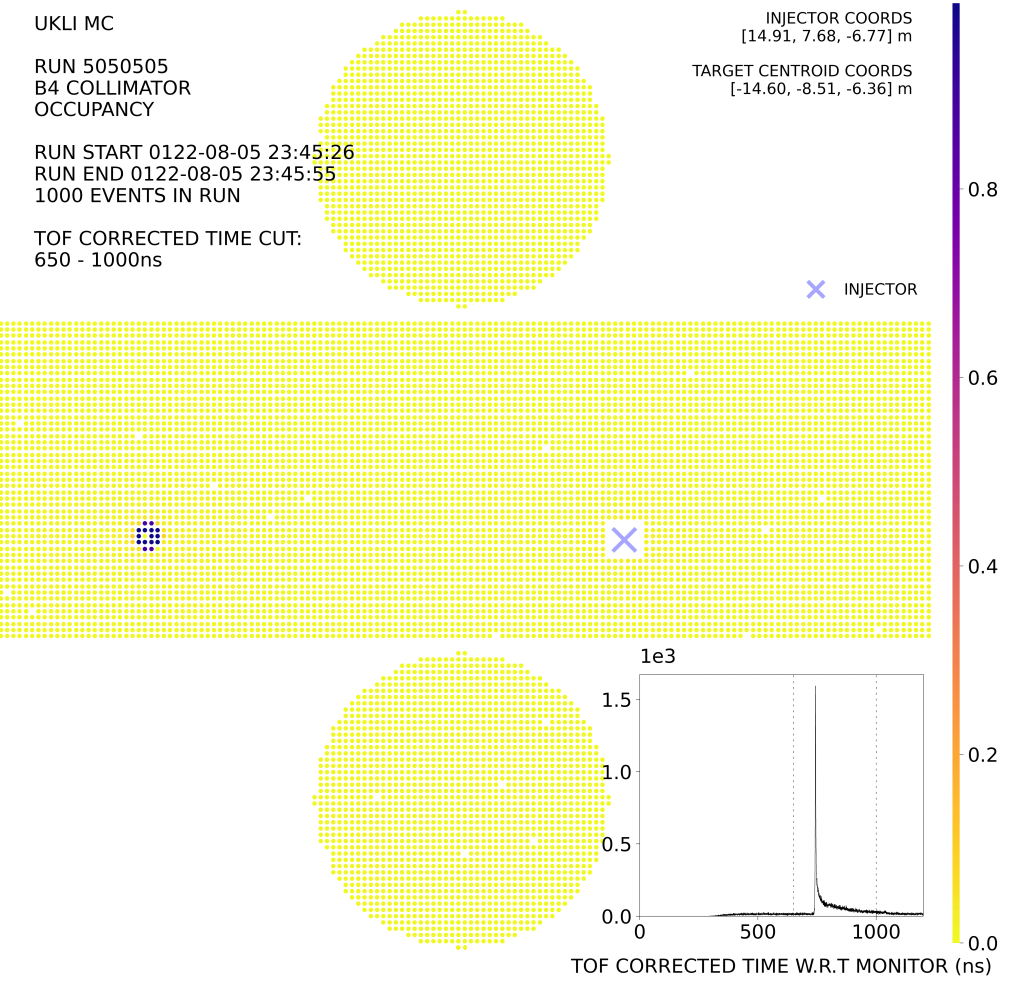
\includegraphics[width=0.9\textwidth]{Figures/ukli_mc_B4.PNG}
    \caption{B4 collimator UKLI MC}
    \label{fig:time4}
    \end{subfigure}
    

    
    \begin{subfigure}{0.49\columnwidth}
    \centering
    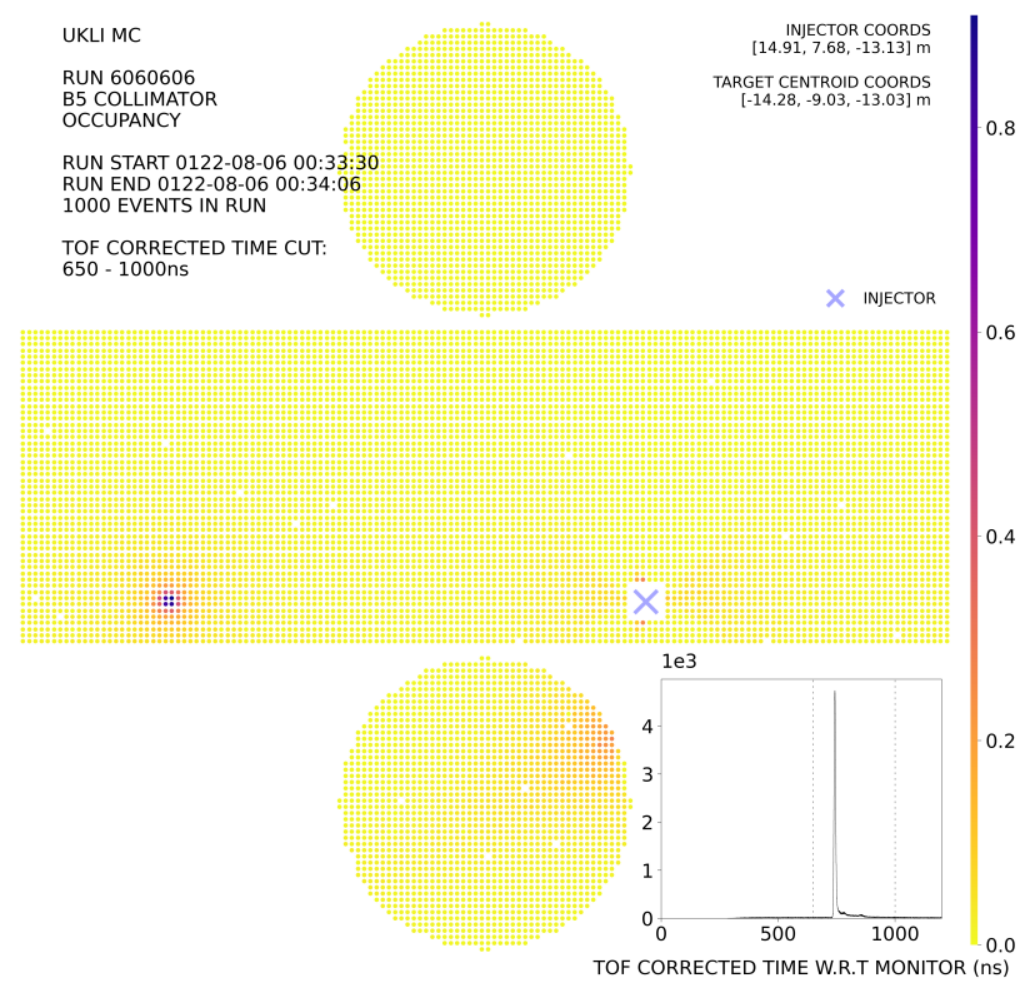
\includegraphics[width=\textwidth]{Figures/ukli_mc_B5.PNG}
    \caption{B5 collimator UKLI MC}
    
    \end{subfigure}

    \end{figure}

    \begin{figure}[htp]
        \centering
        \caption{Monte Carlo simulations of the B1 - B5 diffuser injectors}
        \label{fig:ukli_mc_diff}
        \begin{subfigure}{0.49\columnwidth}
        \centering
        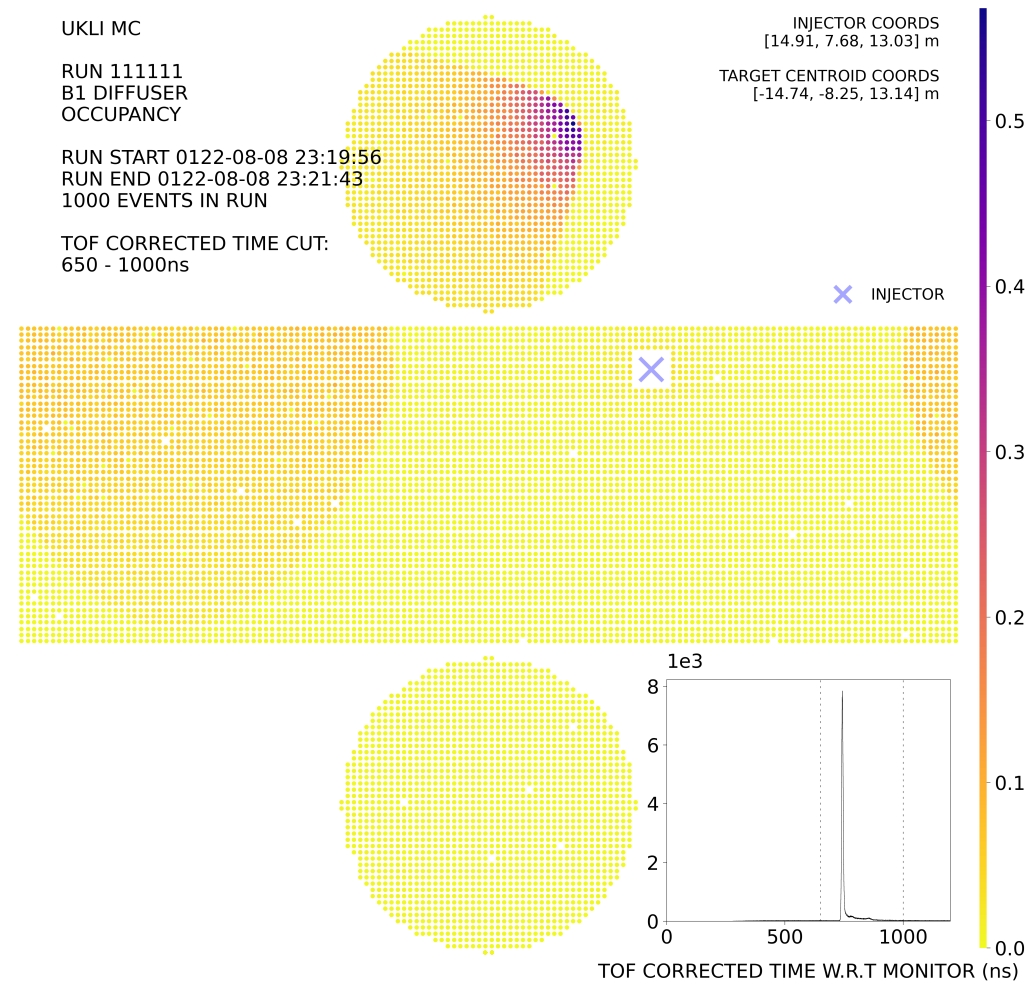
\includegraphics[width=\textwidth]{Figures/ukli_diff_mc_B1.PNG}
        \caption{B1 diffuser UKLI MC}
        \label{fig:time1}
        \end{subfigure}\hfill
        \begin{subfigure}{0.49\columnwidth}
        \centering
        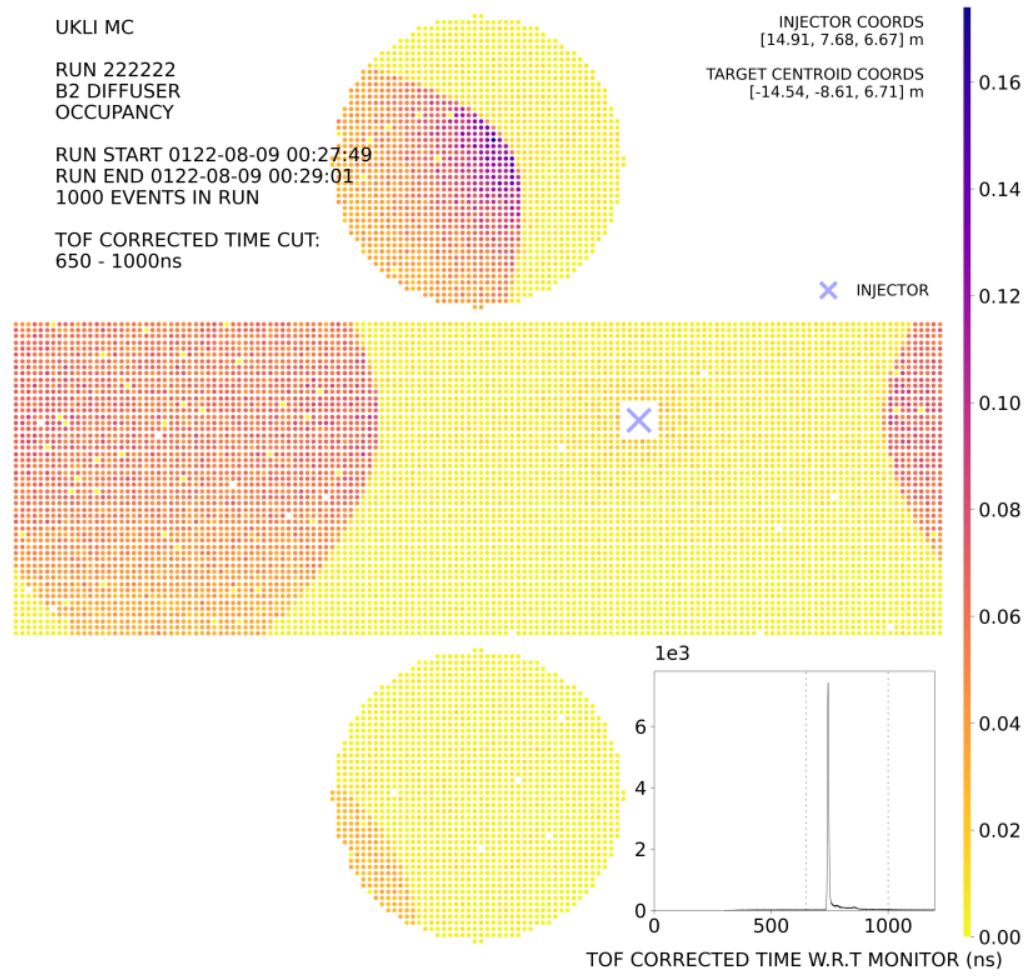
\includegraphics[width=\textwidth]{Figures/ukli_diff_mc_B2.PNG}
        \caption{B2 diffuser UKLI MC}
        \label{fig:time2}
        \end{subfigure}
        
 
        
        \begin{subfigure}{0.49\columnwidth}
        \centering
        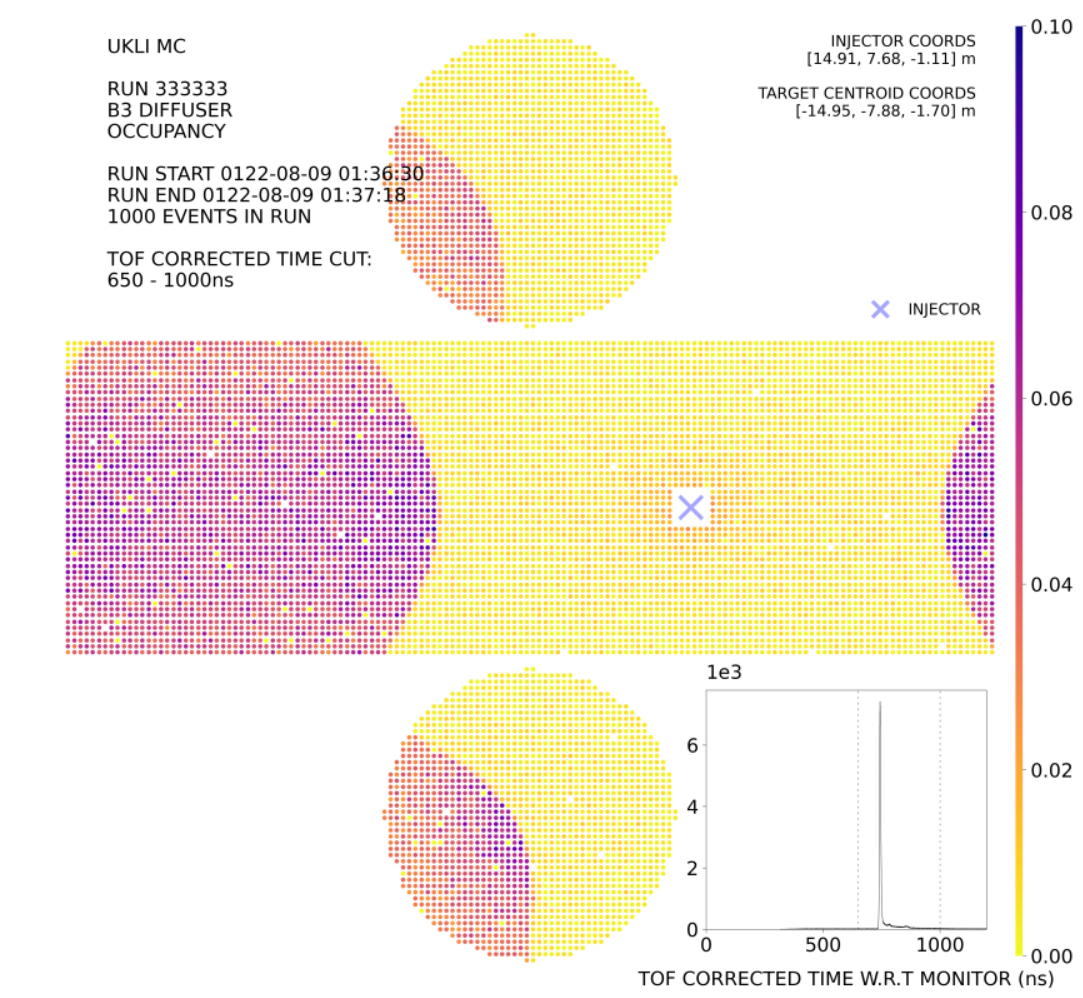
\includegraphics[width=\textwidth]{Figures/ukli_diff_mc_B3.PNG}
        \caption{B3 diffuser UKLI MC}
        \label{fig:time3}
        \end{subfigure}\hfill
        \begin{subfigure}{0.49\columnwidth}
        \centering
        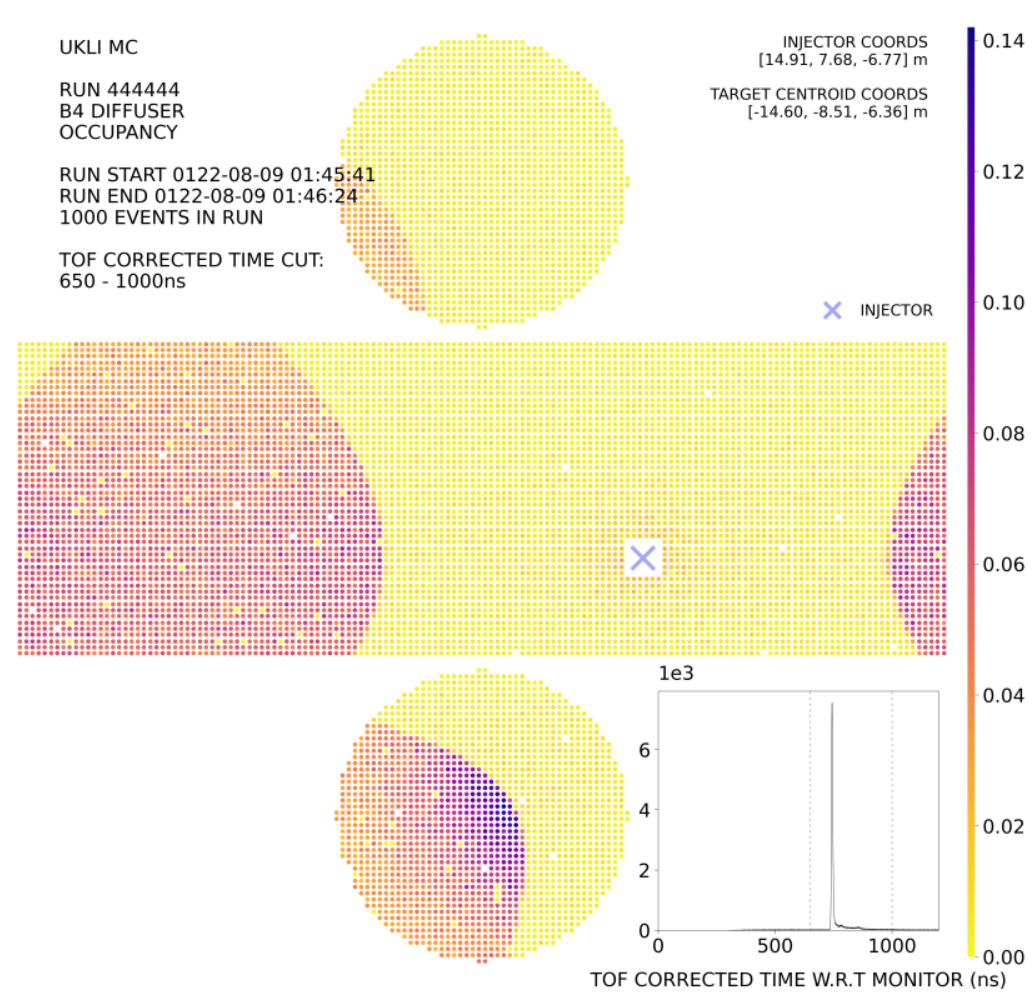
\includegraphics[width=\textwidth]{Figures/ukli_diff_mc_B4.PNG}
        \caption{B4 diffuser UKLI MC}
        \label{fig:time4}
        \end{subfigure}
        
     
        
        \begin{subfigure}{0.49\columnwidth}
        \centering
        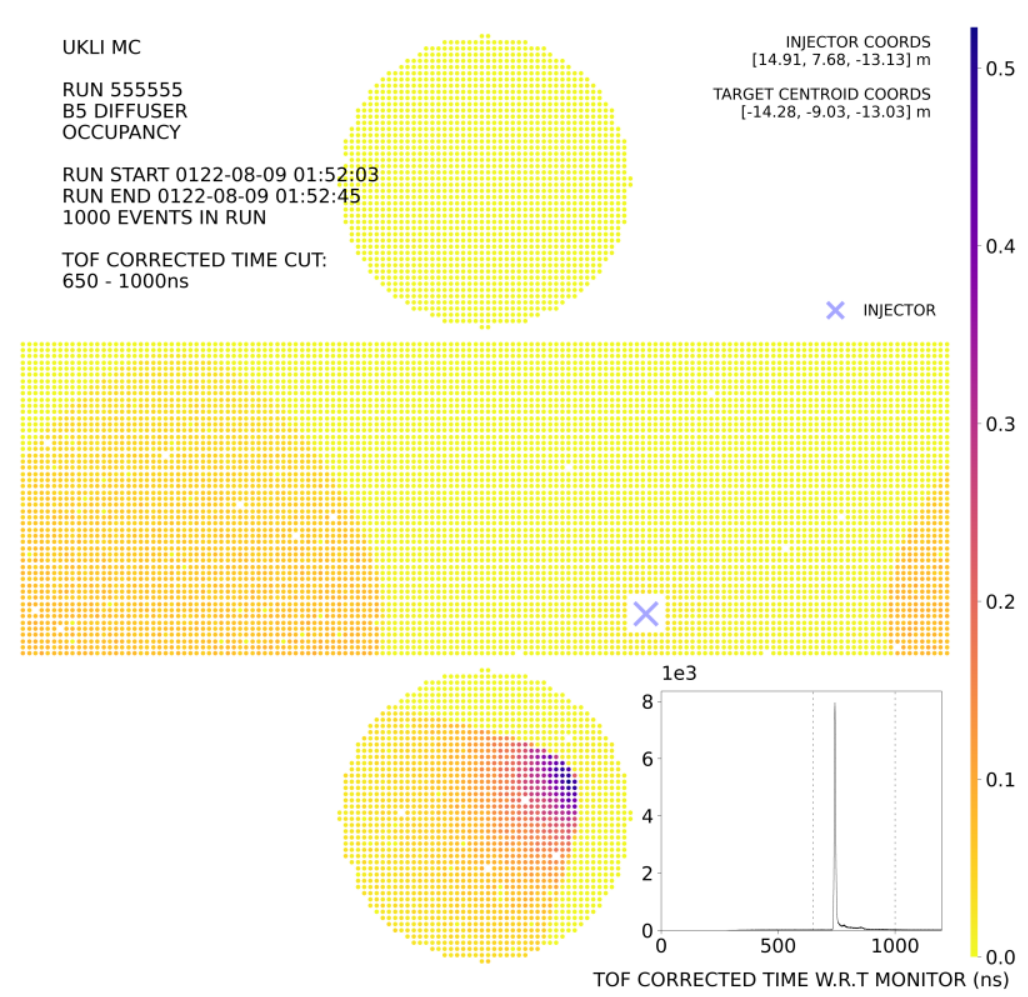
\includegraphics[width=\textwidth]{Figures/ukli_diff_mc_B5.PNG}
        \caption{B5 diffuser UKLI MC}
        
        \end{subfigure}
    
        \end{figure}
    


In order to validate the diffuser MC inverse cumulative distribution function output, a uniform distribution was run through the equation for the diffuser inverse CDF fits and the original PDF fit for each diffuser was used to fit the output points from the distribution, showing that inverse transform sampling was done correctly for the PDFs. These are shown for each diffuser in Figure \ref{fig:inv_cdf_check}. 



\begin{figure}[htp]
    \centering
    \caption{Inverse CDF checks of the B1 - B5 diffusers}
    \label{fig:inv_cdf_check}
    \begin{subfigure}{0.49\columnwidth}
    \centering
    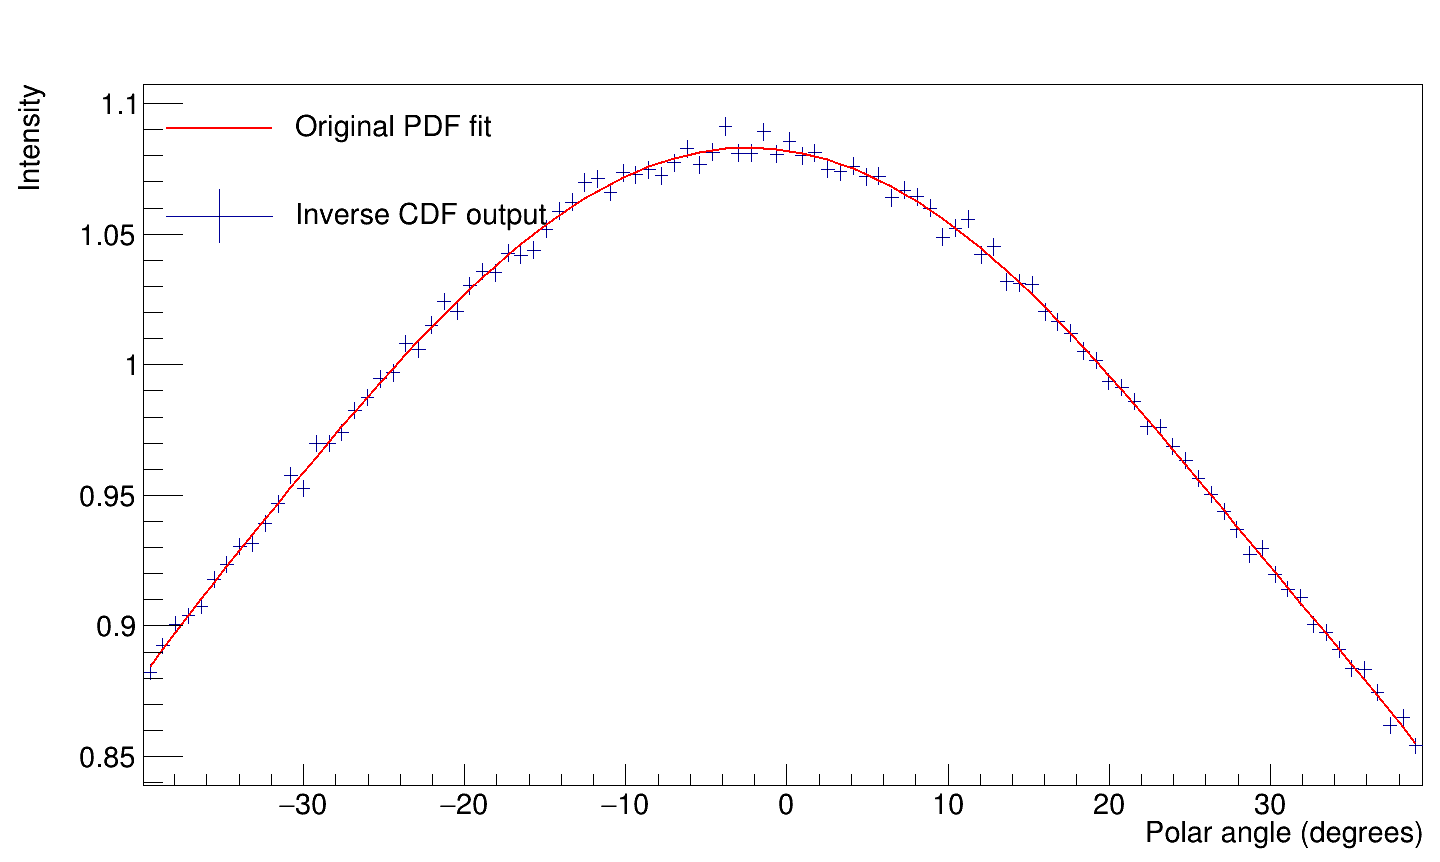
\includegraphics[width=\textwidth]{Figures/inv_cdf_check_diff_B1.PNG}
    \caption{B1 diffuser inverse CDF check}
    \label{fig:time1}
    \end{subfigure}\hfill
    \begin{subfigure}{0.49\columnwidth}
    \centering
    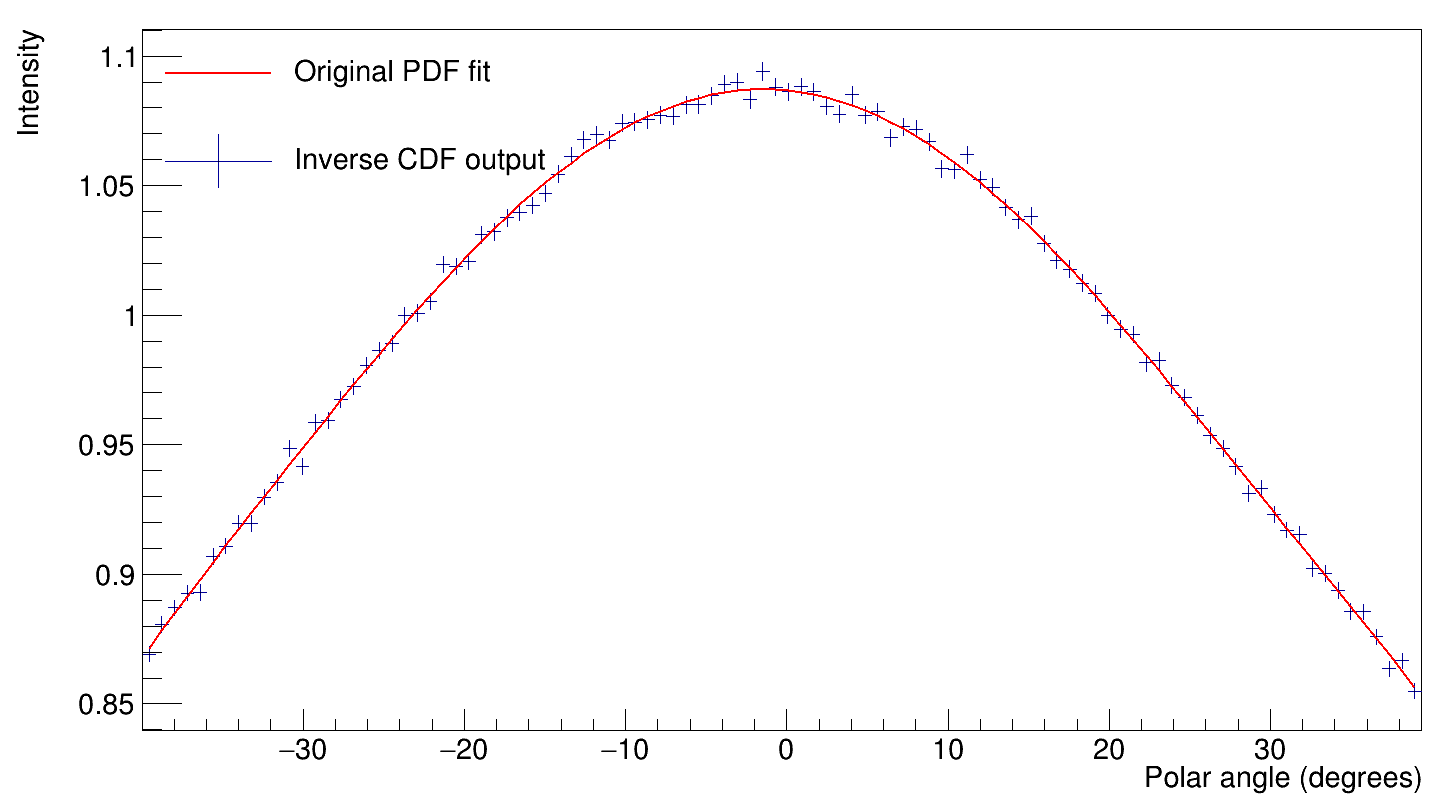
\includegraphics[width=\textwidth]{Figures/inv_cdf_check_diff_B2.PNG}
    \caption{B2 diffuser inverse CDF check}
    \label{fig:time2}
    \end{subfigure}
    
    \medskip
    
    \begin{subfigure}{0.49\columnwidth}
    \centering
    \includegraphics[width=\textwidth]{Figures/inv_cdf_check_diff_B3.PNG}
    \caption{B3 diffuser inverse CDF check}
    \label{fig:time3}
    \end{subfigure}\hfill
    \begin{subfigure}{0.49\columnwidth}
    \centering
    \includegraphics[width=\textwidth]{Figures/inv_cdf_check_diff_B4.PNG}
    \caption{B4 diffuser inverse CDF check}
    \label{fig:time4}
    \end{subfigure}
    
    \medskip
    
    \begin{subfigure}{0.49\columnwidth}
    \centering
    \includegraphics[width=\textwidth]{Figures/inv_cdf_check_diff_B5.PNG}
    \caption{B5 diffuser inverse CDF check}
    
    \end{subfigure}

    \end{figure}


After producing the UKLI MC, the next step was to use them to measure the absorption and scattering parameters in a similar way to the Korean system. As mentioned earlier, this was done by producing time of flight corrected hit timing plots for UKLI MC with multiple different values of absorption, and Rayleigh and Mie scattering parameters and comparing them to the TOF corrected plots for UKLI data. Figures \ref{fig:TOF_abs}, \ref{fig:TOF_ray} and \ref{fig:TOF_mie} show the time-of-flight corrected plots for the UKLI MC B1 collimator, produced with values of the ``abs'' and ``ray'' calibration script parameter between 0.7 and 1.3 to show the affect that varying these parameters have on the time of flight corrected hits. The y-axis shows the number of hits normalised by the total charge in the detector.

\begin{figure}
    \centering
    \includegraphics[width=\textwidth]{Figures/TOF_abs.PNG}
    \caption{Corrected TOF plot with varied absorption, while rayleigh and mie scattering is set to 1.0}
    \label{fig:TOF_abs}
\end{figure}

\begin{figure}
    \centering
    \includegraphics[width=\textwidth]{Figures/TOF_ray.PNG}
    \caption{Corrected TOF plot with varied Rayleigh scattering, while absorption and Mie scattering is set to 1.0}
    \label{fig:TOF_ray}
\end{figure}

\begin{figure}
    \centering
    \includegraphics[width=\textwidth]{Figures/TOF_mie.PNG}
    \caption{Corrected TOF plot with varied Mie scattering, while absorption and Rayleigh scattering is set to 1.0}
    \label{fig:TOF_mie}
\end{figure}

As shown in Figure \ref{fig:TOF_ray}, the TOF corrected timing plots are most affected by the Rayleigh scattering parameter, which affects the amount of hits in the scattered hits region, while varying the absorption parameter mostly affects the height of the reflected peak, as the higher the amount of absorption in the tank, the smaller the number of reflected hits. 

After producing time-of-flight corrected plots for the B1 collimator UKLI MC and overlaying it with the Run 82181 November test run data with the abs, ray, mie parameters set to 1.0, and a TBA value of 7.598, it was clear that there were disgreements between the Monte Carlo and data in both the scattered hits region and the reflected hits peak. In order to change this, the time dispersion of the reflected hits peak was varied, in order to shift the distribution and better match up the UKLI Monte Carlo and test run data. 

The time dispersion for the injected photons in the laser generation in SKDETSIM is governed by a Gaussian distributed random number generated using a Box-Muller transform, where additional time dispersion added would be the sigma of this Gaussian, and after a random number is passed through it, the output number would be added to the time for each track step of the photon giving the time dispersion.

The Box-Muller transform is a random number sampling method for making pairs of independent, normally distributed random sources from a source of uniformly distributed numbers (from between usually from between 0 and 1) \cite{10.1214/aoms/1177706645}. The form of the Box-Muller method implemented to calculate the added time dispersion is the Marsaglia polar method \cite{doi:10.1137/1006063}, which works by choosing two independent and uniformly distributed numbers (u,v) between [-1,+1], so that $s = u^{2} + v^{2}$, and if $s=0$, or $s>=1$, another pair of numbers are chosen. Then the standard normal deviate which is given by $$z_{0}=u \cdot \sqrt{\frac{-2 \ln s}{s}}$$ is multiplied by the chosen value of time dispersion in seconds and added to the mean (set to zero) to give the normally dispersed extra track step time for a photon in the distribution. 

Figure \ref{fig:gauss_time_dispersion} shows the effect of implementing this varying time dispersion on the raw hit timing output from the UKLI MC B1 collimator simulation, with the time dispersion shown for 0 ns, 5 ns, 10 ns, 15 ns, 20 ns and 100 ns. 

\begin{figure}
    \centering
    \includegraphics[width=\textwidth]{Figures/gauss_time_dispersion.PNG}
    \caption{Gaussian distributed time dispersion plots, with varying amounts of time dispersion}
    \label{fig:gauss_time_dispersion}
\end{figure}

Along with implementing the Gaussian distributed time dispersion, introducing a double gaussian for the time dispersion was also looked at, due to the height and sharpness of the reflected peak in the data being something that might be better suited to such a fit. Figure \ref{fig:double_gauss_time_dispersion} shows the raw hit timing output from the UKLI MC B1 collimator simulation with a double gaussian time dispersion, for varying time dispersion values. The x-axis on the plots show the hit time in nanoseconds, the y axis is number of hits. 

\begin{figure}
    \centering
    \includegraphics[width=\textwidth]{Figures/double_gauss_time_dispersion.PNG}
    \caption{Double gaussian distributed time dispersion plots, with varying amounts of time dispersion}
    \label{fig:double_gauss_time_dispersion}
\end{figure}

Figure \ref{fig:TOF_inj} shows the time-of-flight corrected plots for the hits from the injector, for various amounts of Gaussian distributed time dispersion: for 0 ns, 5 ns, 10 ns, 20 ns and 30 ns. 

\begin{figure}
    \centering
    \includegraphics[width=\textwidth]{Figures/TOF_inj.PNG}
    \caption{Gaussian distributed time dispersion plots for the injected hits}
    \label{fig:TOF_inj}
\end{figure}

Figures \ref{fig:5ns_time_dispersion}, \ref{fig:10ns_time_dispersion}, \ref{fig:15ns_time_dispersion}, \ref{fig:20ns_time_dispersion} show time-of-flight corrected time to target hit plots with both a gaussian and double gaussian time dispersion put in for varying amounts of time dispersion for 5, 10, 15 and 20 ns respectively.


\begin{figure}
    \centering
    \includegraphics[width=\textwidth]{Figures/time_dispersion_TOF_5ns.PNG}
    \caption{Gaussian and double gaussian time dispersion for 5ns for the B1 collimator TOF comparison between UKLI MC and Run 82181 test data}
    \label{fig:5ns_time_dispersion}
\end{figure}

\begin{figure}
    \centering
    \includegraphics[width=\textwidth]{Figures/time_dispersion_TOF_10ns.PNG}
    \caption{Gaussian and double gaussian time dispersion for 10ns for the B1 collimator TOF comparison between UKLI MC and Run 82181 test data}
    \label{fig:10ns_time_dispersion}
\end{figure}

\begin{figure}
    \centering
    \includegraphics[width=\textwidth]{Figures/time_dispersion_TOF_15ns.PNG}
    \caption{Gaussian and double gaussian time dispersion for 15ns for the B1 collimator TOF comparison between UKLI MC and Run 82181 test data}
    \label{fig:15ns_time_dispersion}
\end{figure}

\begin{figure}
    \centering
    \includegraphics[width=\textwidth]{Figures/time_dispersion_TOF_20ns.PNG}
    \caption{Gaussian and double gaussian time dispersion for 20ns for the B1 collimator TOF comparison between UKLI MC and Run 82181 test data}
    \label{fig:20ns_time_dispersion}
\end{figure}


For the scattered hits region (region between the dashed lines), there is now good agreement between the MC and data, with this region giving Chi2/NDF values of less than one, and the time dispersion values of 5 ns and 10 ns giving the best agreement. A problem remains regarding the reflected hits peak, where the data continues to have a much higher reflected peak than the Monte Carlo. This points to the amount of charge in the detector for the reflected peak being too large for the Monte Carlo, and further studies will be needed to be done to tune this. These differences are most likely due to misunderstanding the optics in Super-Kamiokande. Future studies will aim to minimise these effects and work towards the installation of a UK Light Injection system in Hyper-Kamiokande with a similar Monte Carlo used to determine absorption and scattering coefficients. 


